%  LaTeX support: latex@mdpi.com 
%  For support, please attach all files needed for compiling as well as the log file, and specify your operating system, LaTeX version, and LaTeX editor.

%=================================================================
\documentclass[journal,article,submit,pdftex,moreauthors]{Definitions/mdpi} 
 

%=================================================================
% MDPI internal commands - do not modify
\firstpage{1} 
\makeatletter 
\setcounter{page}{\@firstpage} 
\makeatother
\pubvolume{1}
\issuenum{1}
\articlenumber{0}
\pubyear{2024}
\copyrightyear{2024}
%\externaleditor{Academic Editor: Firstname Lastname}
\datereceived{ } 
\daterevised{ } % Comment out if no revised date
\dateaccepted{ } 
\datepublished{ } 
%\datecorrected{} % For corrected papers: "Corrected: XXX" date in the original paper.
%\dateretracted{} % For corrected papers: "Retracted: XXX" date in the original paper.
\hreflink{https://doi.org/} % If needed use \linebreak
%\doinum{}
% Esto es para poder escribir acentos directamente:
 
\usepackage{lscape} 
\usepackage{pdflscape}
\usepackage{array} 
\usepackage{longtable} 
 
%% Paquetes de la AMS
\usepackage{amsmath, amsthm, amsfonts}
%% Para añadir archivos con extensión pdf, jpg, png or tif
\usepackage{graphicx}
\usepackage[colorinlistoftodos]{todonotes}
\usepackage[colorlinks=true, allcolors=blue]{hyperref}
 
%=================================================================
% Full title of the paper (Capitalized)
\Title{Revisión sistemática de la literatura sobre Patrimonios Arquitectónicos de Ecuador}

% MDPI internal command: Title for citation in the left column
\TitleCitation{Title}

% Author Orchid ID: enter ID or remove command
\newcommand{\orcidauthorA}{0000-0000-0000-000X} % Add \orcidA{} behind the author's name
%\newcommand{\orcidauthorB}{0000-0000-0000-000X} % Add \orcidB{} behind the author's name

% Authors, for the paper (add full first names)
\Author{Iza Maria $^{1,\dagger,\ddagger}$\orcidA{}{},Macias Rolando$^{2,\ddagger}$ Yela  Jalissath $^{3,\ddagger}$ y Zagal Leslie $^{4,}$*}
%\longauthorlist{yes}

% MDPI internal command: Authors, for metadata in PDF
\AuthorNames{Firstname Lastname, Firstname Lastname and Firstname Lastname}

% MDPI internal command: Authors, for citation in the left column
\AuthorCitation{Lastname, F.; Lastname, F.; Lastname, F.}
% If this is a Chicago style journal: Lastname, Firstname, Firstname Lastname, and Firstname Lastname.

% Affiliations / Addresses (Add [1] after \address if there is only one affiliation.)
\address{%
$^{1}$ \quad Universidad Técnica Estatal de Quevedo; mizam@uteq.edu.ec$^{1}$, rmaciasm3@uteq.edu.ec$^{2}$,jyelat2@uteq.edu.ec$^{3}$,lzagalf@uteq.edu.ec$^{4}$ }
 
% The commands \thirdnote{} till \eighthnote{} are available for further notes

%\simplesumm{} % Simple summary

%\conference{} % An extended version of a conference paper
 
% Abstract (Do not insert blank lines, i.e. \\) 
 
\abstract{\textit{\normalsize The richness and diversity of Ecuador's Architectural Heritage reflects centuries of history, culture and tradition. From the colonial churches to the traditional houses of the different regions of the country, each structure tells a unique and significant story. This review highlights the importance of understanding and preserving these monuments, not only as outstanding examples of architecture, but also as fundamental elements of the country's cultural identity. By analyzing the predominant architectural styles, the cultural and symbolic elements present, as well as the challenges and opportunities associated with their conservation and management, a comprehensive vision of Ecuador's heritage wealth is offered. The systematic review of the literature on Architectural Heritage of Ecuador focuses on the identification of the characteristics, both architectural, historical and cultural, of the different monuments and buildings representative of the country. In addition, the challenges and opportunities associated with its conservation and management are carefully analyzed, considering aspects such as the implementation of rehabilitation programs, the promotion of cultural tourism and community participation in its preservation. Through the formulation of specific research questions, the predominant architectural styles in Ecuador are explored, their connection with the design and structure of heritage, as well as the cultural and symbolic elements present in these constructions and their meaning for the community. Rigorous methodological procedures include the identification of key terms, the search in scientific databases and the careful selection of relevant articles, with the aim of providing a complete and updated view of the state of knowledge on the Architectural Heritages of Ecuador. This systematic review seeks to contribute to the understanding and effective preservation of these important elements of Ecuadorian cultural heritage.} }

% Keywords
\keyword{Architectural heritages; conservation; management; culture and identity} 
 

%%%%%%%%%%%%%%%%%%%%%%%%%%%%%%%%%%%%%%%%%%
 \begin{document}

%%%%%%%%%%%%%%%%%%%%%%%%%%%%%%%%%%%%%%%%%%

% The order of the section titles is different for some journals. Please refer to the "Instructions for Authors” on the journal homepage.

\section{Introducción}

La conservación y valorización de los patrimonios arquitectónicos se presentan como desafíos fundamentales y a la vez enriquecedores para la sociedad moderna \cite{art:articulo1}. Estos esfuerzos no solo se enfocan en la preservación de estructuras y conjuntos urbanos de significado histórico, cultural y estética, sino también promover la historia de nuestras raíces y evolución como civilización \cite{art:articulo2}. Creando así una línea de tiempo entre el ayer y hoy, en el cual cada edificación conservada y espacio urbano relatan historias de eras pasadas, proporcionando lecciones que pueden guiar las acciones actuales y futuras en la arquitectura\cite{art:articulo3}.

En este ámbito, Ecuador se destaca como un escenario privilegiado, dado su diverso legado arquitectónico, que abarca desde ruinas precolombinas hasta la arquitectura colonial y las expresiones modernas \cite{art:articulo4}.  La riqueza del patrimonio arquitectónico ecuatoriano es un reflejo de la complejidad cultural del país, marcada por la diversidad étnica, geográfica y social \cite{art:articulo5}. Cada elemento preservado, ya sea un edificio, una plaza o un conjunto urbano, representa la historia de Ecuador, desde las antiguas construcciones incas y pre-incas que presentan la sofisticación y el poder de estas civilizaciones, hasta las elegantes iglesias y plazas coloniales que hablan de los procesos de colonización y mestizaje, o las innovadoras obras de arquitectura contemporánea que se proyectan hacia el futuro \cite{art:articulo6}.

El creciente interés de proteger y promover el patrimonio arquitectónico ecuatoriano surge como  la necesidad de conservar la identidad cultural del país en el contexto de la globalización y los rápidos cambios urbanos. A pesar de los  esfuerzos por salvaguardar este legado, persisten desafíos relacionados con la conservación efectiva y la integración de estas edificaciones en el ambito de la vida moderna, asegurando que mantenga su relevancia histórica y cultural \cite{art:articulo7}.

El propósito de esta revisión sistemática de la literatura es identificar las características arquitectónicas, históricas y culturales distintivas de los patrimonios arquitectónicos de Ecuador, así como examinar los desafíos y oportunidades vinculados a su conservación y gestión. Para alcanzar este fin, se plantea una pregunta de investigación general: ¿Cuáles han sido las oportunidades para la conservación y gestión de los patrimonios arquitectónicos ecuatorianos?
\par % 
Para abordar esta pregunta general, se formulan tres preguntas de investigación específicas: 
\begin{itemize}
\item ¿Cuáles fueron los estilos arquitectónicos predominantes en los patrimonios arquitectónicos de Ecuador y cómo se reflejaron en su diseño y estructura?
\item ¿Qué elementos culturales y simbólicos estuvieron presentes en los patrimonios arquitectónicos ecuatorianos y cómo contribuyeron a su identidad y significado para la comunidad?
\item ¿Cuáles fueron las oportunidades existentes para la conservación y gestión de los patrimonios arquitectónicos ecuatorianos, como la implementación de programas de rehabilitación, la promoción del turismo cultural o la participación comunitaria en su preservación?
\end{itemize}

%%%%%%%%%%%%%%%%%%%%%%%%%%%%%%%%%%%%%%%%%%
\section{Trabajos Relacionados}
El patrimonio arquitectónico de Ecuador no solo es un conjunto de estructuras físicas, sino que también representa la historia, las tradiciones y la identidad cultural de la nación. Desde edificios coloniales hasta las modestas viviendas rurales, cada estructura cuenta una historia única sobre la evolución social, económica y política del país a lo largo de los siglos \cite{art:articulo9}. Las investigaciones realizadas por expertos como Sagbaicela y otros \cite{art:articulo10}, han mostrado la importancia de conservar y valorar estos bienes arquitectónicos como parte integral del legado cultural ecuatoriano. Estos monumentos no solo son testimonios de la arquitectura de épocas pasadas, sino que también sirven como puntos de referencia históricos y símbolos de orgullo nacional. La preservación de este patrimonio no solo es una cuestión de mantener estructuras físicas, sino también de proteger la memoria colectiva de la sociedad ecuatoriana y de transmitir su rica herencia cultural a las generaciones futuras. 

La preservación de estos patrimonios no solo es una cuestión de mantener estructuras físicas, sino también de proteger la memoria colectiva de la sociedad ecuatoriana y de transmitir su rica herencia cultural a las generaciones futuras \cite{art:articulo11}. En un mundo cada vez más globalizado, el patrimonio arquitectónico local desempeña un papel crucial en la preservación de la diversidad cultural y en la afirmación de la identidad nacional frente a las influencias externas \cite{art:articulo12}. Por lo tanto, es fundamental que se implementen políticas y acciones efectivas para salvaguardar estos tesoros arquitectónicos, asegurando así que continúen siendo una fuente de inspiración y orgullo para las futuras generaciones de ecuatorianos.

Varios estudios, entre ellos el realizado por Hidalgo y Milanes \cite{art:articulo13}, se han dedicado a examinar el estado de conservación de estos bienes en diversas regiones del país. Estas investigaciones no solo ofrecen un panorama de la situación actual de los monumentos y edificaciones históricas, sino que también identifican los desafíos y amenazas específicas que enfrentan. Desde la degradación causada por factores climáticos hasta el deterioro provocado por la falta de mantenimiento, estos estudios arrojan luz sobre las múltiples formas en que el patrimonio arquitectónico ecuatoriano está en riesgo. Asimismo, proporcionan recomendaciones concretas y acciones prácticas para mejorar la protección y la conservación de estos bienes, incluyendo medidas de restauración, políticas de gestión del patrimonio y programas de sensibilización pública\cite{art:articulo14}.  

La expansión urbana y el crecimiento económico han generado una presión sobre el patrimonio arquitectónico en Ecuador. Este fenómeno ha sido objeto de estudio en investigaciones como la realizada por Barsallo \cite{art:articulo15}, la cual se centra en el análisis del impacto de la urbanización en la degradación y pérdida de las edificaciones históricas en el país. Este estudio revela cómo el desarrollo acelerado de las áreas urbanas ha llevado a la demolición o modificación de estructuras históricas para dar paso a nuevas construcciones o infraestructuras modernas. Asimismo, Barsallo destaca cómo la falta de regulaciones adecuadas y la presión del mercado inmobiliario han contribuido a esta situación, poniendo en riesgo la integridad del patrimonio arquitectónico ecuatoriano. Esto resalta la necesidad de implementar políticas de planificación urbana que incorporen la conservación del patrimonio como un elemento fundamental. Dichas políticas deben promover un desarrollo sostenible que proteja y valore la herencia arquitectónica del país, integrando de medidas de conservación y regulación del uso del suelo en los planes de ordenamiento territorial.

El involucrar a la comunidad en la preservación del patrimonio arquitectónico se muestra como un tema de investigación contemporánea. Investigaciones como la realizada por Zamora \cite{art:articulo16}, presentan estrategias de participación en las comunidades locales para la protección y gestión del patrimonio arquitectónico. Este estudio resalta la importancia de la participación comunitaria en los proyectos de conservación, ya que las comunidades locales no solo poseen un conocimiento de la historia y significado de las edificaciones patrimoniales, sino que también tienen un vínculo emocional y cultural con estos sitios. 

García \cite{art:articulo17}, destaca cómo la participación activa de la comunidad puede contribuir a la identificación de problemas de conservación, la formulación de soluciones adaptadas a las necesidades locales y la promoción de un sentido de responsabilidad compartida hacia el patrimonio arquitectónico. Además, el estudio evidencia cómo la participación comunitaria puede fortalecer el sentido de pertenencia hacia los bienes patrimoniales, lo que a su vez fomenta prácticas de conservación sostenibles a largo plazo. En este sentido, la importancia de promover mecanismos de participación inclusivos que permitan la colaboración activa entre la comunidad, las instituciones gubernamentales, organizaciones no gubernamentales y otros actores relevantes. Estos mecanismos deben fomentar el diálogo, la transparencia y la equidad en la toma de decisiones relacionadas con la conservación del patrimonio arquitectónico, garantizando que las voces de todas las partes interesadas sean escuchadas y tenidas en cuenta.

La protección y gestión del patrimonio arquitectónico en Ecuador se encuentran ligadas al papel de las instituciones gubernamentales, una temática abordada por investigaciones como la realizada por Tenze \cite{art:articulo18}. Este estudio se centra en la evaluación del marco legal e institucional relacionado con la conservación del patrimonio en el país, arrojando luz sobre las fortalezas y debilidades de la legislación y las políticas públicas vigentes. La investigación de Tenze ofrece una mirada detallada sobre cómo las instituciones gubernamentales están estructuradas para abordar la protección del patrimonio arquitectónico, examinando los mecanismos legales y las estrategias de gestión implementadas.  

La promoción de la conservación del patrimonio arquitectónico en Ecuador no solo se limita a acciones gubernamentales y políticas, sino que también implica un importante esfuerzo en educación y sensibilización pública. Este aspecto ha sido ampliamente abordado en investigaciones como la realizada por Aguirre \cite{art:articulo21}, la cual desempeña un papel en la promoción de una cultura de valoración y respeto hacia el patrimonio histórico del país. Los programas educativos analizados no solo proporcionan conocimientos sobre la historia y el valor del patrimonio arquitectónico, sino que también fomentan actitudes proactivas hacia su protección y conservación.

El análisis del turismo cultural como un recurso financiero para la conservación del patrimonio arquitectónico en Ecuador ha sido objeto de investigación en diversos estudios, entre los cuales el trabajo de Cárdenas \cite{art:articulo19}, examina el impacto del turismo en la conservación y promoción de sitios históricos y monumentos arquitectónicos en el contexto ecuatoriano, así como sus implicaciones en términos de sostenibilidad y gestión. Cárdenas identifica cómo el turismo cultural ha generado una fuente de ingresos destinados a la conservación y restauración de edificaciones patrimoniales en Ecuador, contribuyendo así a su preservación a largo plazo. Sin embargo, Cárdenas también señala los desafíos asociados con el turismo cultural, como la presión sobre los recursos naturales y culturales, el riesgo de sobreexplotación de los sitios patrimoniales y la necesidad de gestionar adecuadamente el flujo turístico para garantizar la sostenibilidad a largo plazo.

El uso de tecnologías de información y comunicación (TIC) en la conservación del patrimonio arquitectónico ha sido objeto de creciente interés en la investigación contemporánea. Zambrano \cite{art:articulo20}, se centra en la exploración de herramientas digitales innovadoras, tales como la fotogrametría y la realidad aumentada, y su aplicación tridimensional y la visualización de edificaciones históricas en el contexto ecuatoriano. Zambrano detalla cómo estas tecnologías pueden contribuir a la preservación  del patrimonio arquitectónico al ofrecer métodos eficientes para la captura de datos y la creación de modelos digitales de alta fidelidad.

A pesar de los avances en la investigación sobre el patrimonio arquitectónico en Ecuador, es evidente que aún existen desafíos que requieren una atención continua y un enfoque multidimensional. Entre estos desafíos se encuentran aspectos relacionados con la conservación y gestión sostenible de este legado cultural \cite{art:articulo22}.  
 
%%%%%%%%%%%%%%%%%%%%%%%%%%%%%%%%%%%%%%%%%%
\section{Materiales y Metodos}
El presente estudio se centra en una revisión sistemática de la literatura sobre los patrimonios arquitectónicos de Ecuador, con el objetivo de explorar los hallazgos y tendencias presentes en la investigación académica sobre este tema. Para llevar a cabo esta investigación, se emplea una metodología } basada en las directrices propuestas por Barbara Kitchenham,  reconocida en el ámbito de la investigación científica. 
Esta metodología es un proceso estructurado que abarca desde la definición de un protocolo de revisión hasta el análisis de los resultados obtenidos. El protocolo de revisión establece los criterios de inclusión y exclusión, las estrategias de búsqueda bibliográfica y los procedimientos para la extracción y síntesis de datos. La búsqueda bibliográfica se llevó a cabo en bases de datos científicas, utilizando términos de  específicos relacionados con el tema de estudio. Posteriormente, se seleccionaron los estudios de acuerdo con los criterios establecidos y se extrajo la información  para su análisis. Esta metodología garantiza la  validez de los resultados, proporcionando una visión actualizada del conocimiento sobre los patrimonios arquitectónicos de Ecuador.
 

\textbf{\subsection{Definición de Protocolo de Revisión}} 
Se elaboró un protocolo de revisión que estableció los objetivos, criterios de inclusión y exclusión, estrategias de búsqueda, y procedimientos de análisis de datos. Este protocolo sirvió durante todo el proceso de revisión, asegurando la coherencia de los resultados. La búsqueda se limitó a los últimos 5 años y se enfocó en artículos publicados en inglés. Se utilizó una variedad de bases de datos científicas, incluyendo  Archnet, MDPI y Sage Open Access.

\textbf{\subsubsection{Búsqueda Bibliográfica Sistemática}}
Se llevó a cabo una búsqueda  de la literatura relevante en las bases de datos científicas mencionadas. Se utilizaron términos de búsqueda específicos relacionados con el tema de estudio, como:
\par
\begin{itemize}
\item ''Ecuadorian architectural heritage''
\item ''Architectural characteristics''
\item ''Historical characteristics''
\item ''Cultural characteristics''
\item ''Conservation challenges''
\item ''Architectural styles in Ecuador''
\item ''Architectural design and structure''
\item ''Cultural and symbolic elements''
\item ''Cultural tourism''
\item ''Community participation in preservation''
\end{itemize}

\textbf{\subsubsection{Criterios de inclusión y exclusión}} 
En los criterios de exclusión, se descartaron aquellos trabajos que no estaban directamente relacionados con la pregunta de investigación para este estudio. Además, se excluyeron los estudios que no contaban con una metodología o con la falta de referencias académicas.  

En cuanto a los criterios de inclusión, se consideraron estudios publicados en los últimos cinco años, escritos en inglés debido a su reconocimiento en el ámbito académico. Se incluyeron investigaciones que abordaban aspectos relacionados con los patrimonios arquitectónicos de Ecuador, como los procedimientos de investigación, la tipología arquitectónica, los estilos y corrientes arquitectónicas, los aspectos culturales incorporados, los materiales utilizados en la construcción, la condición de preservación y los desafíos y problemas de preservación.

\textbf{\subsubsection{Selección de Estudios}} 
 La selección de artículos se realizó mediante una revisión basada en los resúmenes de los estudios y buscando información en bases de datos académicas, como  Archnet, MDPI y Sage Open Access. Posteriormente, se evaluaron en detalle los estudios preseleccionados, analizando la relevancia de cada investigación.

\textbf{\subsubsection{ Extracción de Datos} } 
Para la extracción de datos, se recopiló información detallada de cada estudio seleccionado. Se extrajeron variables como:
\begin{itemize}
\item Procedimientos de investigación empleados
\item Tipología arquitectónica abordada
\item Estilos y corrientes arquitectónicas
\item Aspectos culturales incorporados en las estructuras
\item Materiales utilizados en la construcción
\item Condición de preservación de los patrimonios arquitectónicos estudiados
\item Desafíos y problemas específicos de preservación identificados
 
\end{itemize}

 Esta información fue registrada de manera sistemática y se utilizó para realizar un análisis de los estudios incluidos en la revisión sistemática.
 
%%%%%%%%%%%%%%%%%%%%%%%%%%%%%%%%%%%%%%%%%%
\section{Resultados y Discusión}
El protocolo de Kitchenham es una metodología ampliamente reconocida y utilizada en la realización de revisiones sistemáticas de la literatura en una variedad de disciplinas académicas. Dentro del contexto del estudio sobre los Patrimonios Arquitectónicos de Ecuador, esta metodología ofrece un marco estructurado y  para llevar a cabo la búsqueda, selección y análisis de la literatura pertinente. 
\newpage
 \begin{landscape}
 \fontsize{7}{10}\selectfont %
\begin{longtable}{|>{\small}c|*{14}{p{1.3cm}|}}
 % aquí añadimos el encabezado de la primera hoja.
 \hline  N &Título del artículo&Tipo de estudio&Revista&Año de publicación&País de origen&Procedimientos de Investigación&Tipología arquitectónica&Estilos y Corrientes Arquitectónicas&Aspectos culturales incorporados&Materiales utilizados en la Construcción&Condición de Preservación&Desafíos y Problemas de Preservación&Estudiante Revisor&Enlace \\
\hline \hline
\endfirsthead
% aquí añadimos el encabezado del resto de hojas.
 \hline N&Título del artículo&Tipo de estudio&Revista&Año de publicación&País de origen&Procedimientos de Investigación&Tipología arquitectónica&Estilos y Corrientes Arquitectónicas&Aspectos culturales incorporados&Materiales utilizados en la Construcción&Condición de Preservación&Desafíos y Problemas de Preservación&Estudiante Revisor
 &Enlace\\
\hline \hline
\endhead
% aquí añadimos el fondo de todas las hojas, excepto de la última.
\multicolumn{14}{c}{Sigue en la página siguiente.}
\endfoot

% aquí añadimos el fondo de la última hoja.
\endlastfoot

1 &Arquitectura, patrimonio y el metaverso &Articulo &Traditional Dwellings and Settlements Review  &2020 &Inglaterra &Revisión crítica de la literatura
Análisis de estudios de casos &Patrimonio arquitectónico (sin especificación) &Arquitectura clásica
Arquitectura moderna
Arquitectura contemporánea &Tradiciones
Rituales
Prácticas sociales&Piedra
Ladrillo
Madera
Hormigón &Deterioro
Estrategias de conservación &Autenticidad
Accesibilidad
Propiedad intelectual &Iza Masapanta Maria Jose & \url{https://www.jstor.org/stable/27074915} \\
\hline
 
2 &Olvido de valores intangibles y comunidad: El caso de las políticas de conservación del patrimonio en Cuenca, Ecuador& Artículo científico& Journal of Urban Management, International Journal of Heritage Studies& 2024& Ecuador& Análisis de políticas de conservación del patrimonio
Examen de valores intangibles y comunitarios
Estudio de casos  & Patrimonio cultural urbano
& Arquitectura colonial
Arquitectura Barroco
Arquitectura Neoclásico& Identidad cultural
Memoria colectiva
Sentido de pertenencia& Adobe
Piedra
Madera& Deterioro
Abandono
Vulnerabilidad& Falta de recursos
Desinterés político
Turismo masivo
Gentrificación
Desconexión entre las políticas públicas y las necesidades de la comunidad& Macias Millingalli Rolando Alexander&\url{https://www.sciencedirect.com/science/article/pii/S2226585623000961}\\
\hline

3 &Geometría y proporciones de los edificios vernáculos de adobe de Cuenca (Ecuador)& Artículo científico& International Journal of Architectural Heritage& 2020& Ecuador& Análisis métrico 
Levantamiento de planos
Análisis de la geometría y proporciones
Entrevistas a expertos
Observación participante& Patrimonio naturales
Patrimonio culturales  
Vivienda vernácula 
Edificios religiosos 
Edificios públicos& Arquitectura Precolombino
Arquitectura Colonial
Arquitectura Republicano& Construcción tradicionales
Técnicas constructivas tradicionales
Valor histórico y cultural & Tapial
Bahareque 
Adobe
Piedra 
Cal
Madera
Teja& Falta de mantenimiento
Riesgo de colapso
Grietas en los muros& Falta de recursos
Desinterés político
Cambio climático
Deterioro del patrimonio
Turismo masivo& Yela Tinitana Jalissath Jareth&\url{https://www.tandfonline.com/doi/abs/10.1080/15583058.2021.1879312}\\
\hline

 4 &Marcos de investigación, metodologías y métodos de evaluación relacionados con la reutilización adaptativa del patrimonio arquitectónico: una revisión &Articulo de revisión &International Journal of Built heritage  &2021 &China &Revisión bibliográfica
Análisis de contenido
Síntesis de la literatura &Patrimonio arquitectónico (sin especificación) &No se mencionan estilos específicos &Valor histórico
Valor social
Sostenibilidad&No se mencionan materiales específicos &Deterioro
Abandono
Vulnerabilidad &Compatibilidad con el valor patrimonial
Integración de nuevas funciones
Financiación &Zagal Figueroa Leslie Monserrate &\url{https://link.springer.com/article/10.1186/s43238-021-00025-x}\\
\hline

5 &Propuesta de geoportal para el inventario del patrimonio cultural en nabón (Ecuador)& Artículo científico& International Journal of Heritage Studies
International Journal of imagery& 2020& Ecuador& Revisión de la literatura
Análisis de experiencias previas
Diseño de un geoportal
Evaluación del geoportal& Patrimonio cultural material (arquitectura, arqueología, bienes muebles)
Patrimonio cultural inmaterial (tradiciones, fiestas, gastronomía)& Arquitectura Colonial
Arquitectura Republicano
Arquitectura Indígena& Técnicas constructivas tradicionales
Valor histórico y cultural& Adobe
Piedra
Madera
Teja
Barro
Quincha
Bambú
Paja& Estado de deterioro avanzado
Falta de mantenimiento& Falta de recursos
Desinterés político
Cambio climático
Deterioro del patrimonio
Turismo masivo& Iza Masapanta Maria Jose&\url{ https://isprs-archives.copernicus.org/articles/XLIII-B2-2020/1415/2020/isprs-archives-XLIII-B2-2020-1415-2020.html}\\ 
\hline

6 &Características Acústicas de los Teatros Patrimoniales de Quito-Ecuador& Artículo científico& Journal Applied Acoustics& 2023& Ecuador& Medición de la acústica en 5 teatros patrimoniales de Quito
Análisis de los resultados
Comparación con los estándares internacionales
Modelado acústico& Teatros a la italiana
Teatros de herradura
Teatros experimentales& Arquitectura Neoclásico
Arquitectura Art Nouveau
Arquitectura Art Deco & Valor histórico y cultural  
Espacios de encuentro y difusión cultural
Símbolos de la ciudad de Quito& Madera
Piedra
Ladrillo
Yeso
Metal
Vidrio
Pintura
Textiles& Deterioro
Vulnerabilidad a desastres
Riesgo de incendio& Intervenciones inadecuadas
Deterioro del patrimonio
Desinterés político& Macias Millingalli Rolando Alexander&\url{https://documentacion.sea-acustica.es/publicaciones/Madeira21/ID8.pdf}\\ 
\hline
 
7 &Una revisión de las herramientas y técnicas utilizadas en la preservación digital del patrimonio arquitectónico dentro de los ciclos de desastres. &Articulo &International Journal Heritage Science &2023 &China &Revisión de la literatura
Análisis comparativo de herramientas y técnicas
Evaluación de casos de estudio &Patrimonio arquitectónico (sin especificación) &No se mencionan estilos específicos &Valor histórico
Valor social
Memoria colectiva&No se mencionan materiales específicos &Deterioro
Daños por desastre
Vulnerabilidad &Precisión de la documentación digital
Accesibilidad
Sostenibilidad a largo plazo &Yela Tinitana Jalissath Jareth &\url{https://link.springer.com/article/10.1186/s40494-023-01035-x}\\ 
\hline

8 &Operabilidad de datos de nubes de puntos en un modelo de información del patrimonio arquitectónico &Articulo de investigación &International Journal of Architectural Heritage  &2021 &España &Revisión de la literatura
Análisis de casos de estudio
Desarrollo de un modelo de información del patrimonio arquitectónico (H-BIM) &Patrimonio arquitectónico (sin especificación) &No se mencionan estilos específicos &Valor histórico
Valor social
Memoria colectiva&No se mencionan materiales específicos &Deterioro
Daños por desastres
Vulnerabilidad &Integración de datos de nubes de puntos en H-BIM
Semantización de datos
Visualización y análisis &Zagal Figueroa Leslie Monserrate &\url{https://www.tandfonline.com/doi/abs/10.1080/15583058.2021.1900951}\\ 
\hline

9 &Por encima de los barrancos: evaluación de la vulnerabilidad a las inundaciones del patrimonio arquitectónico de tierra en Quito (Ecuador) &Articulo &Natural Hazards and Geomorphology &2022 &España, Ecuador &Evaluación de la vulnerabilidad
Análisis multicriterio
Método Delphi &Patrimonio arquitectónico de tierra
Edificios históricos
Viviendas tradicionales &Arquitectura colonial
Arquitectura vernácula &Valor histórico
Valor social
Identidad cultural&Tierra
Adobe
Tapial &Deterioro
Vulnerabilidad a las inundaciones
Riesgo de colapso &Mitigación del riesgo de inundaciones
Reforzamiento estructural
Rehabilitación sostenible &Iza Masapanta Maria Jose &\url{https://www.mdpi.com/2076-3417/12/23/11932}\\
\hline

10 &Metodología de gestión BIM para la documentación de proyectos de restauración arquitectónica: Estudio de caso de Cuenca-Ecuador &Articulo de investigación &API Conference Proceedings &2022 &Ecuador &Gestión BIM
Documentación arquitectónica
Levantamiento 3D
Modelado BIM &Patrimonio arquitectónico (sin especificación)
Edificios históricos &No se mencionan estilos específicos. &Valor histórico
Valor social
Memoria colectiva&No se mencionan materiales específicos. &Deterioro
Necesidad de intervención &Precisión de la documentación
Interoperabilidad de software
Capacitación profesional &Macias Millingalli Rolando Alexander &\url{https://pubs.aip.org/aip/acp/article-abstract/2574/1/090004/2830070}\\
\hline

11 &Rehabilitación de la Casa Gillespie para Oficinas de Gestión Patrimonial en Quito, Ecuador& Articulo de investigación& Journal of Architectural Conservation& 2023& Ecuador& Análisis histórico y arquitectónico de la Casa Gillespie
Estudio de las técnicas constructivas tradicionales
Levantamiento de planos
Diseño de la rehabilitación
Ejecución de la obra & Vivienda unifamiliar
Edificio patrimonial& Arquitectura Art Nouveau
Arquitectura Eclecticismo& Valor histórico y cultural 
Diseño arquitectónico
Materiales de construcción tradicionales
Técnicas constructivas tradicionales& Piedra
Ladrillo
Madera
Metal
Vidrio
Pintura
Yeso
Cerámica& Algunos signos de deterioro
Desprendimiento de la pintura 
Pudrición de la madera& Deterioro del patrimonio
Falta de conocimiento
Intervenciones inadecuadas
Falta de recursos& Yela Tinitana Jalissath Jareth&\url{https://www.taylorfrancis.com/chapters/edit/10.1201/9781003136804-48/rehabilitation-guillespie-house-heritage-management-offices-quito-ecuador-l%C3%B3pez-ulloa"}\\
\hline

12 &Caracterización del patrimonio construido de centros históricos orientada a la evaluación de su vulnerabilidad sísmica: El caso de Cuenca, Ecuador &Articulo de investigación &International Journal of Disaster Risk Reduction &2022 &Ecuador &Caracterización geométrica
Análisis de materiales
Clasificación tipológica
Evaluación sísmica &Patrimonio edificado (sin especificación) &Arquitectura colonial
Arquitectura republicana
Arquitectura vernácula &Valor histórico 
Valor social
Memoria colectiva
Identidad cultural&Adobe
Tapial
Madera
Piedra &Deterioro
Vulnerabilidad sísmica
Riesgo de colapso &Mitigación del riesgo sísmico
Reforzamiento estructural
Rehabilitación sostenible
Gestión del riesgo de desastres &Zagal Figueroa Leslie Monserrate &\url{https://www.sciencedirect.com/science/article/abs/pii/S2212420922000036}\\
\hline

13 &Una propuesta sustentable para una declaración de patrimonio cultural en Ecuador: la vivienda vernácula de Portoviejo &Artículo científico &International Journal of Sustainability &2022 &Ecuador  &Investigación cualitativa
Entrevistas semiestructuradas
Historias de vida
Observación científica
Análisis de contenido &Vivienda vernácula
Vivienda tradicional
Arquitectura popular &No se mencionan estilos específicos. &Identidad cultural
Tradiciones
Valores sociales
Usos y costumbres&Materiales naturales
Madera
Adobe
Bambú &Deterioro
Vulnerabilidad a desastres
Necesidad de intervención &Protección del patrimonio cultural
Desarrollo sostenible
Rehabilitación de viviendas
Transmisión de conocimientos &Iza Masapanta Maria Jose &\url{https://www.mdpi.com/2071-1050/15/2/1115}\\
\hline

14 &Protocolos técnicos de conservación patrimonial desde el análisis de riesgos y vulnerabilidades. El caso de la arquitectura vernácula de Quingeo (Azuay, Ecuador) &Artículo científico &Revista de Arqueología de la arquitectura &2023 &Ecuador  &Análisis de riesgos y vulnerabilidades
Matriz de análisis de riesgos
Estratigrafía muraria
Principios de la conservación preventiva &Arquitectura vernácula
Edificios históricos &No se mencionan estilos específicos. &Valor histórico
Valor social
Identidad cultural&Adobe
Tapial
Madera
Piedra &Deterioro
Vulnerabilidad a desastres
Necesidad de intervención &Mitigación de riesgos
Reforzamiento estructural
Rehabilitación sostenible
Gestión del patrimonio &Macias Millingalli Rolando Alexander &\url{https://arqarqt.revistas.csic.es/index.php/arqarqt/article/view/302}\\
\hline

15 & Plan de conservación preventiva para la capilla de susudel, Ecuador& Articulo de conferencia internacional& International Journal of Heritage & 2020& Ecuador 
España& Análisis histórico y arquitectónico de la Capilla de Susudel
Estudio de las técnicas constructivas tradicionales
Levantamiento de planos
Diagnóstico del estado de conservación
Propuesta de un plan de conservación preventiva& Edificio religioso
Capilla& Arquitectura Colonial
Arquitectura Barroco& Valor histórico y cultural 
Diseño arquitectónico
Materiales de construcción tradicionales
Técnicas constructivas tradicionales& Adobe
Piedra
Madera
Teja
Ladrillo
Yeso
Barro
Quincha& Algunos signos de deterioro
Desprendimiento de la teja 
Pudrición de la madera& Deterioro del patrimonio
Falta de conocimiento
Intervenciones inadecuadas & Yela Tinitana Jalissath Jareth&\url{ https://isprs-archives.copernicus.org/articles/XLIV-M-1-2020/811/2020/isprs-archives-XLIV-M-1-2020-811-2020.pdf}\\
\hline

16 &Consideraciones sobre la Vulnerabilidad del Patrimonio Arquitectónico. Estudio de caso: la Iglesia de El Sagrario, Cuenca, Ecuador &Artículo científico &Journal Intervención (Mexico DF) &2020 &Mexico, Ecuador &Revisión bibliográfica,
Análisis de mecanismos de daño en edificaciones tipo iglesia
Aplicación de metodología italiana para evaluación de vulnerabilidad
Estudio de caso de la Iglesia de El Sagrario. &Patrimonio arquitectónico (sin especificación) &No se mencionan estilos específicos. &Atributos históricos
Artísticos y de antigüedad como elementos culturales asociados al sitio patrimonial&Tierra &Evaluación de la vulnerabilidad &Vulnerabilidad sísmica &Zagal Figueroa Leslie Monserrate &\url{https://www.scielo.org.mx/scielo.php?pid=S2007-249X2020000100257&script=sci_arttext&tlng=en}\\
\hline

17 &El rol de la universidad en el mantenimiento de las edificaciones de patrimonio vernáculo en la región sur del Ecuador &Artículo científico &Book Preventive Conservation - From Climate and Damage Monitoring to a Systemic &2020 &Ecuador &No se menciona  &Patrimonio vernáculo
Edificaciones patrimoniales &Arquitectura vernácula
No se mencionan estilos específicos. &Identidad cultural
Tradiciones
Valores sociales
Usos y costumbres&Materiales naturales
Adobe
Tapial
Madera &Deterioro
Vulnerabilidad a desastres
Necesidad de intervención &Mantenimiento del patrimonio
Capacitación
Investigación
Difusión
Financiación &Iza Masapanta Maria Jose &\url{https://books.google.es/books?hl=es&lr=&id=0ynvDwAAQBAJ&oi=fnd&pg=PA103&dq=Ecuadorian+architectural+heritage&ots=8-aOKc3xYv&sig=NBfNHYNwsgfnbdeF_zx8P_mTXTE#v=onepage&q=Ecuadorian%20architectural%20heritage&f=false} \\
\hline

18 & El papel de la universidad en el mantenimiento de edificios patrimoniales vernáculos en la región sur de Ecuador& Articulo de investigación& International Journal of Heritage Management and Conservation& 2020& Ecuador& Revisión de la literatura
Análisis de experiencias previas
Encuestas a expertos
Estudio de casos& Vivienda vernácula
Edificios religiosos
Edificios públicos& Arquitectura Colonial
Arquitectura Republicano
Arquitectura Indígena& Materiales de construcción tradicionales 
Técnicas constructivas tradicionales
Valor histórico y cultural& Adobe
Piedra
Madera
Teja
Barro
Quincha
Bambú
Paja & Falta de mantenimiento
Desprendimiento de la teja 
Pudrición de la madera& Deterioro del patrimonio
Falta de conocimiento
Intervenciones inadecuadas
Falta de recursos& Macias Millingalli Rolando Alexander&\url{https://www.taylorfrancis.com/chapters/edit/10.1201/9781003004042-15/role-university-maintaining-vernacular-heritage-buildings-southern-region-ecuador-garc%C3%ADa-tenze-achig}\\
\hline

19 & Estimación de Pérdidas para Fachadas Típicas de Adobe de Cuenca (Ecuador) ante Escenarios de Sismo& Artículo científico& International Journal of Architectural Heritage& 2021& España, Ecuador& Análisis numérico de las fachadas de adobe
Modelado del comportamiento sísmico
Estimación de las pérdidas económicas
Evaluación de la vulnerabilidad sísmica& Vivienda vernácula
Edificios históricos& Arquitectura Colonial
Arquitectura Republicano& Materiales de construcción tradicionales 
Técnicas constructivas tradicionales
Valor histórico y cultural & Adobe
Madera
Teja
Piedra
Cal
Arena
Tierra
Agua & Estado avanzado de deterioro
Vulnerabilidad sísmica 
Falta de mantenimiento& Deterioro del patrimonio
Falta de conocimiento
Intervenciones inadecuadas & Yela Tinitana Jalissath Jareth&\url{https://www.tandfonline.com/doi/abs/10.1080/15583058.2021.1977417}\\
\hline

20 &Arquitectura moderna en el discurso profesional: análisis del archivo de la Bienal de Quito 1976-1992 utilizando redes bipartitas& Artículo científico& Journal Digital Scholarship in the Humanities& 2021& Ecuador& Análisis del archivo de la Bienal de Quito 1976-1992
Construcción de redes bipartitas
Análisis de las relaciones entre actores, temas y proyectos
Identificación de los principales discursos sobre arquitectura moderna& Patrimonio pública
Patrimonio de Arquitectura privada
Vivienda& Arquitectura Modernismo
Arquitectura Brutalismo
Arquitectura Postmodernismo& Valor histórico y cultural 
Diseño arquitectónico
Materiales de construcción modernos 
Técnicas constructivas modernas& Hormigón
Vidrio
Acero
Ladrillo
Madera
Piedra
Metal
Pintura & Estado de abandono & Deterioro del patrimonio
Falta de conocimiento
Presión urbana& Zagal Figueroa Leslie Monserrate&\url{https://www.researchgate.net/profile/Patricia-Acosta-Vargas/publication/355955312_Modern_architecture_in_the_professional_discourse_analysis_of_the_Architectural_Biennial_of_Quito's_1976-92_archive_using_bipartite_networks/links/6186156ad7d1af224bb9b51a/Modern-architecture-in-the-professional-discourse-analysis-of-the-Architectural-Biennial-of-Quitos-1976-92-archive-using-bipartite-networks.pdf"
 https://www.mdpi.com/2571-9408/5/4/207}\\
\hline

21 &Un puente sin nombre: La resignificación controvertida del patrimonio arquitectónico urbano desde una perspectiva de género en Cuenca (Ecuador) &Artículo científico &International Journal of Heritage Studies &2023 &España, Ecuador &Estudio de caso
Análisis documental
Entrevistas a expertos &Edificios públicos
Espacios públicos &Arquitectura Colonial
Arquitectura Republicano &Género
Identidad
Memoria&Piedra
Ladrillo
Madera &Regular
Deterioro &Falta de recursos
Desinterés político
Vandalismo &Iza Masapanta Maria Jose &\url{https://www.mdpi.com/2571-9408/6/5/233}\\
\hline

22 &Una experiencia de promoción de la cultura constructiva vernácula en Susudel (Ecuador) &Artículo científico &International Archives of the Photogrammetry, Remote Sensing and Spatial Information Sciences &2020 &Ecuador &Talleres participativos con la comunidad
Análisis de la arquitectura vernácula
Documentación de las técnicas tradicionales &Viviendas vernáculas
Edificios comunitarios &Arquitectura Vernáculo
Arquitectura Andino &Materiales de construcción tradicionales
Técnicas constructivas tradicionales
Cosmovisión andina&Adobe
Piedra
Madera &Deterioro
Necesidad de intervención &Falta de recursos
Desinterés político
Materiales de construcción modernos &Macias Millingalli Rolando Alexander &\url{https://isprs-archives.copernicus.org/articles/XLIV-M-1-2020/623/2020/isprs-archives-XLIV-M-1-2020-623-2020.html}\\
\hline

23 &El contexto del Patrimonio Mundial de Ecuador, para estrategias de desarrollo sostenible &Artículo científico &International Journal of Design and Nature and Ecodynamics &2020 &Ecuador &Análisis documental
Revisión bibliográfica
Estudio de caso &Sitios naturales
Sitios culturales &Arquitectura Precolombino
Arquitectura Colonial
Arquitectura Republicano &Diversidad cultural
Identidad
Memoria&Piedra
Adobe
Madera &Deterioro
Vulnerabilidad a desastres
Necesidad de intervención &Falta de recursos
Desinterés político
Cambio climático &Yela Tinitana Jalissath Jareth &\url{https://www.researchgate.net/profile/Nataly-Paz/publication/339817915_The_Context_of_Ecuador's_World_Heritage_for_Sustainable_Development_Strategies/links/604d5dbd458515e529a79d07/The-Context-of-Ecuadors-World-Heritage-for-Sustainable-Development-Strategies.pdf}\\
\hline

24 & Caracterización y Análisis de los Morteros de la Iglesia de Santo Domingo en Quito (Ecuador) &Artículo científico &International Journal of Architectural Heritage
 &2020 &Ecuador & Análisis petrográfico de los morteros
Análisis físico-químico de los morteros
Ensayos mecánicos de los morteros
Estudio de la composición química
Estudio de la microestructura 
 &Edificio religioso
Iglesia
 &Arquitectura Colonial
Arquitectura Barroco &Valor histórico y cultural 
Diseño arquitectónico
Materiales de construcción tradicionales 
Técnicas constructivas modernas
 & Piedra
Ladrillo
Madera
Cal
Arena
Agua
Yeso
Pigmentos 
&Algunos signos de deterioro
Pudrición de la madera
& Falta de recursos
Desinterés político
Vandalismo 
 &Zagal Figueroa Leslie Monserrate &\url{https://www.mdpi.com/2571-9408/5/4/207}\\
\hline

25 &Fiesta “La Tejería”: influencia en la arquitectura vernácula de Poaló. Píllaro. Ecuador &Artículo científico &International Journal of Heritage Science &2022 &Ecuador & Observación participante en la Fiesta de La Tejería
Análisis de las formas arquitectónicas de las viviendas
Entrevistas a los habitantes de Poaló
Revisión de la literatura sobre arquitectura vernácula  &Patrimonio vernácula
Patrimonio religiosos
 & Arquitectura Colonial
Arquitectura Republicano
Arquitectura Indígena 
 & Materiales de construcción tradicionales
Técnicas constructivas tradicionales
Cosmovisión andina
Simbolismo
Ritos y tradiciones 
 & Adobe
Teja
Madera
Piedra
Ladrillo
Barro
Quincha
Paja  &Algunos signos de deterioro 
Grietas en los muros
Desprendimiento de la teja 
Pudrición de la madera & Intervenciones inadecuadas
Deterioro del patrimonio
Falta de conocimiento 
 &Iza Masapanta Maria Jose & \url{https://revistascientificas.cuc.edu.co/moduloarquitecturacuc/article/download/3435/3410/24519}\\
\hline

26 &Experiencias de participación social en la recuperación del patrimonio vernáculo en el sur de Ecuador &Artículo científico &International Journal of Heritage Studies &2020 &Ecuador &Estudio de caso
Análisis de experiencias
Entrevistas a actores clave &Viviendas vernáculas
Edificios comunitarios &Arquitectura Vernáculo
Arquitectura Andino &Materiales de construcción tradicionales
Técnicas constructivas tradicionales
Cosmovisión andina &Adobe
Piedra
Madera &Regular
Deterioro &Falta de recursos
Desinterés político
Materiales de construcción modernos &Macias Millingalli Rolando Alexander &\url{https://isprs-archives.copernicus.org/articles/XLIV-M-1-2020/603/2020/isprs-archives-XLIV-M-1-2020-603-2020.html}\\
\hline

27 &Potencial del patrimonio cultural como aporte al desarrollo turístico de Montecristi, Ecuador &Artículo científico &Revista Espacios, Journal of Vytautas Magnus University &2020 &Ecuador &Investigación descriptiva
Análisis documental
Trabajo de campo &Patrimonio tangible e intangible
Manifestaciones culturales
Sitios históricos &Arquitectura Colonial
Arquitectura Republicano
Arquitectura Vernáculo &Tradiciones
Costumbres
Artesanías &Adobe
Piedra
Madera &Deterioro
Vulnerabilidad a desastres
Necesidad de intervención &Falta de recursos
Desinterés político
Vandalismo &Yela Tinitana Jalissath Jareth &\url{https://versita.com/menuscript/index.php/Versita/article/view/1498/1508}\\
\hline

28 &Técnicas de documentación geomática como herramientas de monitoreo para el patrimonio rural construido en Nabón (Ecuador) &Artículo científico & International Journal of Architectural Heritage &2020 &Ecuador &Documentación geomática
Monitoreo del patrimonio
Análisis de datos &Edificios religiosos
Edificios civiles &Arquitectura vernácula
Arquitectura Colonial
Arquitectura Republicano &Materiales de construcción tradicionales
Técnicas constructivas tradicionales
Cosmovisión andina &Adobe
Piedra
Madera &Deterioro
Vulnerabilidad a las inundaciones
Riesgo de colapso &Falta de recursos
Desinterés político
Materiales de construcción modernos &Zagal Figueroa Leslie Monserrate &\url{https://isprs-annals.copernicus.org/articles/VIII-M-1-2021/65/2021/isprs-annals-VIII-M-1-2021-65-2021.html}\\
\hline

29 &Consideraciones sobre la vulnerabilidad del patrimonio arquitectónico. Estudio de caso: la iglesia de El Sagrario, Cuenca, Ecuadoe& Artículo científico& Revista Internacional de Conservación, Restauración y Museología& 2020& Ecuador& Revisión bibliográfica
Estudio de mecanismos de colapso en terremotos pasados
Extrapolación de conocimientos y experiencias
Análisis de vulnerabilidad sísmica y daños en inmuebles religiosos
Aplicación de metodología italiana para identificación de macroelementos
Mecanismos de daño en inmuebles tipo iglesia& Patrimonio cultural y religioso& No se mencionan estilos específicos.& Identidad cultural y religioso& Tierra
Piedra
Madera& Deterioro
Vulnerabilidad a desastres 
 & Prevenir daños por actividad sísmica
Prevención de desastres
Impactos en el patrimonio arquitectónico& Iza Masapanta Maria Jose&\url{https://oa.upm.es/65794/1/INVE_MEM_2020_323541.pdf}\\
\hline

30 &Ruinas de haciendas como sitios de memoria difícil en Chimborazo, Ecuador &Artículo científico &Journal of Latin American Cultural Studies &2020 &Ecuador &Análisis documental
Estudio de caso
Entrevistas a actores clave &Ruinas de haciendas
Sitios patrimoniales &Arquitectura Colonial
Arquitectura Republicano &Sistema de hacienda
Explotación laboral
Lucha social &Adobe
Piedra
Madera &Ruinas
Deterioro &Falta de recursos
Desinterés político
Vandalismo &Macias Millingalli Rolando Alexander &\url{https://journals.sagepub.com/doi/abs/10.1177/1469605314521275}\\
\hline

31 &Fotogrametría y Realidad Aumentada para Promover el Patrimonio Cultural Religioso de la Catedral de San Pedro en Guayaquil, Ecuador &Artículo científico &International Journal of Heritage Studies &2023 &Ecuador &Fotogrametría
Realidad aumentada
Desarrollo de prototipo &Edificios religiosos
Patrimonio cultural &Arquitectura Neogótico &Religión católica
Arte sacro
Historia &Piedra
Ladrillo
Madera &Bueno &Deterioro natural
Falta de recursos
Vandalismo &Yela Tinitana Jalissath Jareth &\url{https://link.springer.com/chapter/10.1007/978-3-030-42520-3_47}\\
\hline

32 &La colonialidad de los paisajes urbanos patrimoniales de la UNESCO: Proceso patrimonial y gentrificación transnacional en Cuenca, Ecuador &Artículo científico &nternational Journal of Urban and Regional Research &2023 &Ecuador &Análisis de documentos
Entrevistas a actores clave
Observación participante &Paisajes urbanos
Patrimonio cultural &Arquitectura Colonial
Arquitectura Republicano &Cosmovisión andina
Tradiciones ancestrales
Identidad cultural &Adobe
Piedra
Madera &Regular
Deterioro &Falta de recursos
Desinterés político
Turismo masivo &Zagal Figueroa Leslie Monserrate &\url{https://journals.sagepub.com/doi/full/10.1177/0042098019888441}\\
\hline

33 &Los desafíos del patrimonio natural y cultural de Galápagos y Quito, Ecuador &Artículo científico &Revista de Estudios Regionales, : Tourism planning and development in Latin America &2023 &Ecuador &Análisis documental
Entrevistas a expertos &Patrimonio natural
Patrimonio cultural &Arquitectura Colonial
Arquitectura Republicano
Arquitectura Moderno &Biodiversidad
Cosmovisión andina
Tradiciones ancestrales &Adobe
Piedra
Madera &Regular
Deterioro &Falta de recursos
Desinterés político
Turismo masivo
Cambio climático &Iza Masapanta Maria Jose &\url{https://www.cabidigitallibrary.org/doi/abs/10.1079/9781789243048.0086}\\
\hline

34 &Desempeño de la iluminación natural en la arquitectura vernácula: estudio de caso del casco antiguo de Pasa, Ecuador &Artículo científico &Energy Conversion and Management: X &2023 &Ecuador &Mediciones de iluminación natural
Análisis de planos y fotografías
Entrevistas a residentes &Arquitectura vernácula
Viviendas &Arquitectura Colonial
Arquitectura Republicano
Arquitectura Vernáculo &Materiales de construcción tradicionales
Técnicas constructivas tradicionales &Adobe
Piedra
Madera &Deterioro
Vulnerabilidad a las inundaciones
Riesgo de colapso &Falta de recursos
Desinterés político
Materiales de construcción modernos &Macias Millingalli Rolando Alexander &\url{https://www.sciencedirect.com/science/article/pii/S2590174523001502}\\
\hline

35 &Valor percibido en un sitio del Patrimonio Mundial de la UNESCO: el caso de Quito, Ecuador &Artículo científico &Journal of Cultural Heritage Management and Sustainable Development  &2022 &Ecuador &Encuesta a visitantes
Análisis de contenido &Sitio patrimonial
Ciudad &Arquitectura Colonial
Arquitectura Republicano &Centro histórico
Iglesias
Monumentos &Piedra
Ladrillo
Madera &Deterioro
Necesidad de intervención &Turismo masivo
Deterioro del patrimonio
Falta de recursos &Yela Tinitana Jalissath Jareth &\url{https://www.emerald.com/insight/content/doi/10.1108/JCHMSD-03-2022-0049/full/html}\\
\hline

36 &Planes Maestros de Patrimonio como Instrumento Técnico para la Preservación y Puesta en Valor del Patrimonio Cultural del Ecuador &Paper &ArTeS: Architecture, Technology and Sustainability &2022 &Ecuador &Análisis documental
Entrevistas a expertos &Instrumento técnico
Gestión del patrimonio &No se mencionan estilos específicos. &No se menciona &No se mencionan materiales específicos.  &Regular
Deterioro &Falta de recursos
Desinterés político
Deterioro del patrimonio
Turismo masivo &Zagal Figueroa Leslie Monserrate &\url{https://revistas.ug.edu.ec/index.php/artes/article/view/1678}\\
\hline

37 &dentidad Visual Basada en Iconografía Ancestral: Una Estrategia para la Revalorización del Patrimonio Cultural Caranqui en el Sitio Arqueológico Gualimán (Ecuador) &Artículo científico &Journal of Heritage &2022 &Ecuador &Análisis documental
Entrevistas a expertos
Diseño de una propuesta de identidad visual &Patrimonio cultural
Arqueología
Turismo cultural &Arquitectura Precolombino
Arquitectura Inca &Cosmovisión andina
Simbolismo ancestral
Cerámica
Tejidos
Orfebrería &Piedra
Adobe
Madera &Regular
Deterioro &Falta de recursos
Desinterés político
Turismo masivo
Falta de promoción &Iza Masapanta Maria Jose &\url{https://www.mdpi.com/2571-9408/5/4/178}\\
\hline

38 &Métodos de Evaluación de la Sostenibilidad en Edificios Existentes: Análisis Comparativo en Bienes Patrimoniales Destinados a Uso Público en Girón, Ecuador &Artículo científico &IOP Conference Series: Materials Science and Engineering &2023 &Ecuador &Análisis documental
Revisión de estudios de caso
Aplicación de métodos de evaluación de la sostenibilidad a dos bienes patrimoniales en Girón &Arquitectura
Patrimonio cultural
Edificios públicos &Arquitectura Colonial
Arquitectura Republicano &Materiales de construcción tradicionales
Técnicas constructivas tradicionales
Valor histórico y cultural &Adobe
Piedra
Madera
Ladrillo &Deterioro
Necesidad de intervención &Falta de recursos
Desinterés político
Deterioro del patrimonio
Turismo masivo
Adaptación a criterios de sostenibilidad &Macias Millingalli Rolando Alexander &\url{https://iopscience.iop.org/article/10.1088/1757-899X/1203/3/032128/meta}\\
\hline

39 &Chamanes del Formativo Tardío en la Costa Ecuatoriana: Evidencia Arquitectónica, Mortuoria y Artefactual de Salango en las Fases Engoroy Medio y Tardío (600–100 a. C.) &Artículo científico &Journal of the Institute of Andean Studies
 &2021 &Ecuador &Excavaciones arqueológicas
Análisis de arquitectura
Análisis de entierros
Análisis de artefactos
Interpretación etnoarqueológica &Arqueología
Sociedad
Religión &Formativo Tardío
Costa ecuatoriana &Chamanismo
Ritualidad
Muerte
Creencias &Adobe
Piedra
Madera
Concha &Regular
Deterioro &Falta de recursos
Desinterés político
Saqueo
Erosión &Yela Tinitana Jalissath Jareth &\url{https://www.tandfonline.com/doi/abs/10.1080/00776297.2020.1834203}\\
\hline

40 &Caracterización y Análisis de los Morteros de la Iglesia de San Francisco de Quito (Ecuador &Artículo científico &Journal of Heritage &2023 &Ecuador &Análisis petrográfico
Análisis físico-químico
Ensayos mecánicos &Arquitectura
Patrimonio cultural
Materiales de construcción &Arquitectura Colonial
Arquitectura Barroco &Materiales de construcción tradicionales
Técnicas constructivas tradicionales
Valor histórico y cultural &Piedra
Ladrillo
Madera
Mortero &Deterioro
Necesidad de intervención &Falta de recursos
Desinterés político
Deterioro del patrimonio
Turismo masivo &Zagal Figueroa Leslie Monserrate &\url{https://www.mdpi.com/2571-9408/6/12/393}\\
\hline
\caption{Tabla de extracción de datos}
\label{tab:fruta}
\end{longtable}
\end{landscape}
\newpage 
\subsection{\textbf{Detalles de artículos} }
Los resultados de esta revisión sistemática de la literatura sobre Patrimonios Arquitectónicos de Ecuador revelan una amplia diversidad de publicaciones que abordan este tema desde diferentes perspectivas y enfoques. Durante nuestro análisis en la figura 1, identificamos un total de 40 trabajos relevantes, los cuales se distribuyen en diversas categorías de tipo de estudio. La mayoría de estos trabajos corresponden a artículos científicos, un total de 30, seguidos por artículos de conferencia internacional (3), artículos de investigación (5), y un artículo de revisión junto con un paper. \par %
\begin{figure} [h!]
    \centering
    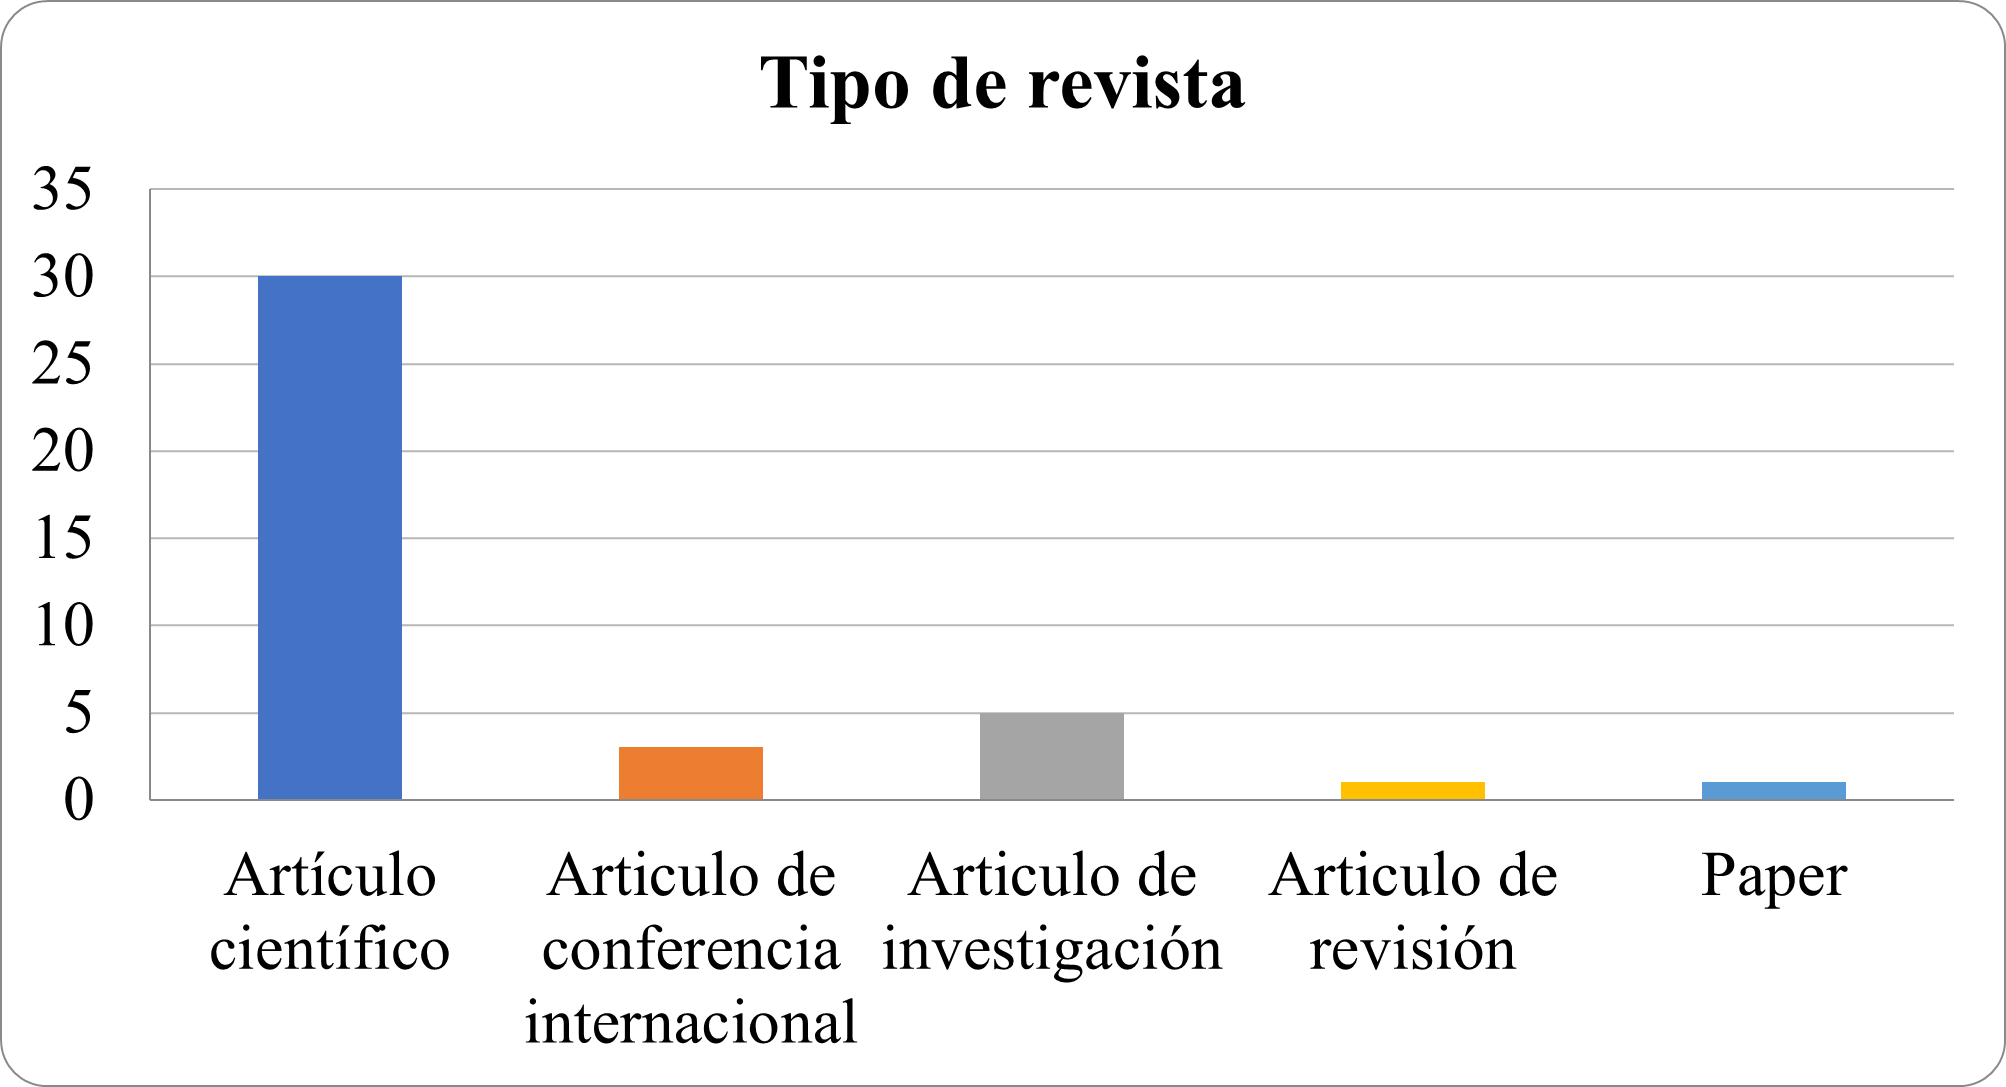
\includegraphics[width=0.8\textwidth]{Graficos/Tipos de revista.png}
    \caption{Tipos de revista}
    \label{fig:grafico}
\end{figure}
    
\par %
El año de publicación de estos trabajos, mostró una distribución variada a lo largo de los últimos años, con un pico notable en el año 2020, donde se publicaron 15 trabajos. Este dato sugiere un creciente interés en la investigación sobre Patrimonios Arquitectónicos de Ecuador en la última década, con una constante producción de conocimiento en este campoc(Figura 2). \par %
\begin{figure} [h!]
  \centering
  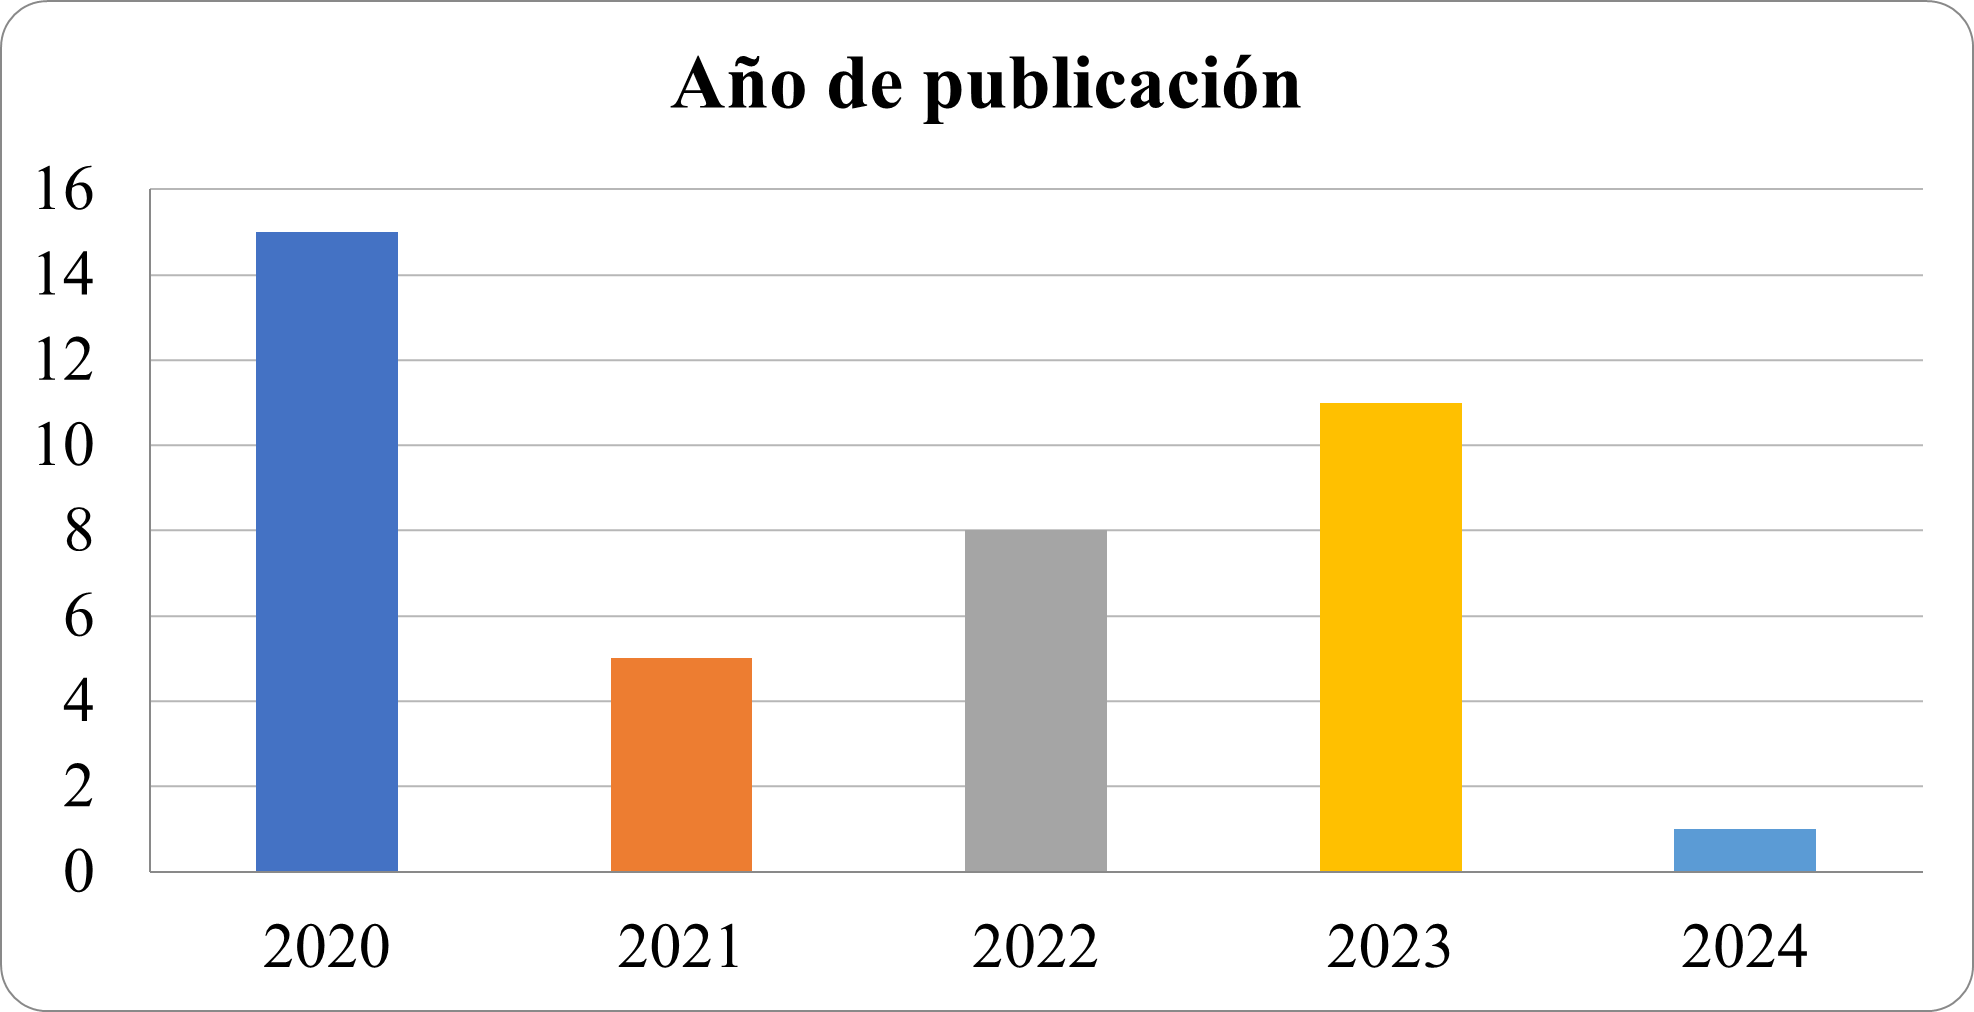
\includegraphics[width=0.9\textwidth]{Graficos/año de publicación.png}
    \caption{Año de publicación}
  \label{fig:grafico}
\end{figure}  
\par %
Respecto al país de origen de las investigaciones. En figura 3 es evidente que Ecuador es el país que lidera en la producción de trabajos sobre este tema, con un total de 31 publicaciones. Le siguen España (5), China (2), México (1) e Inglaterra (1). Este hallazgo resalta la importancia y el interés local en la preservación y estudio del patrimonio arquitectónico nacional.
\newpage
\par %
  \begin{figure} [h!]
    \centering
    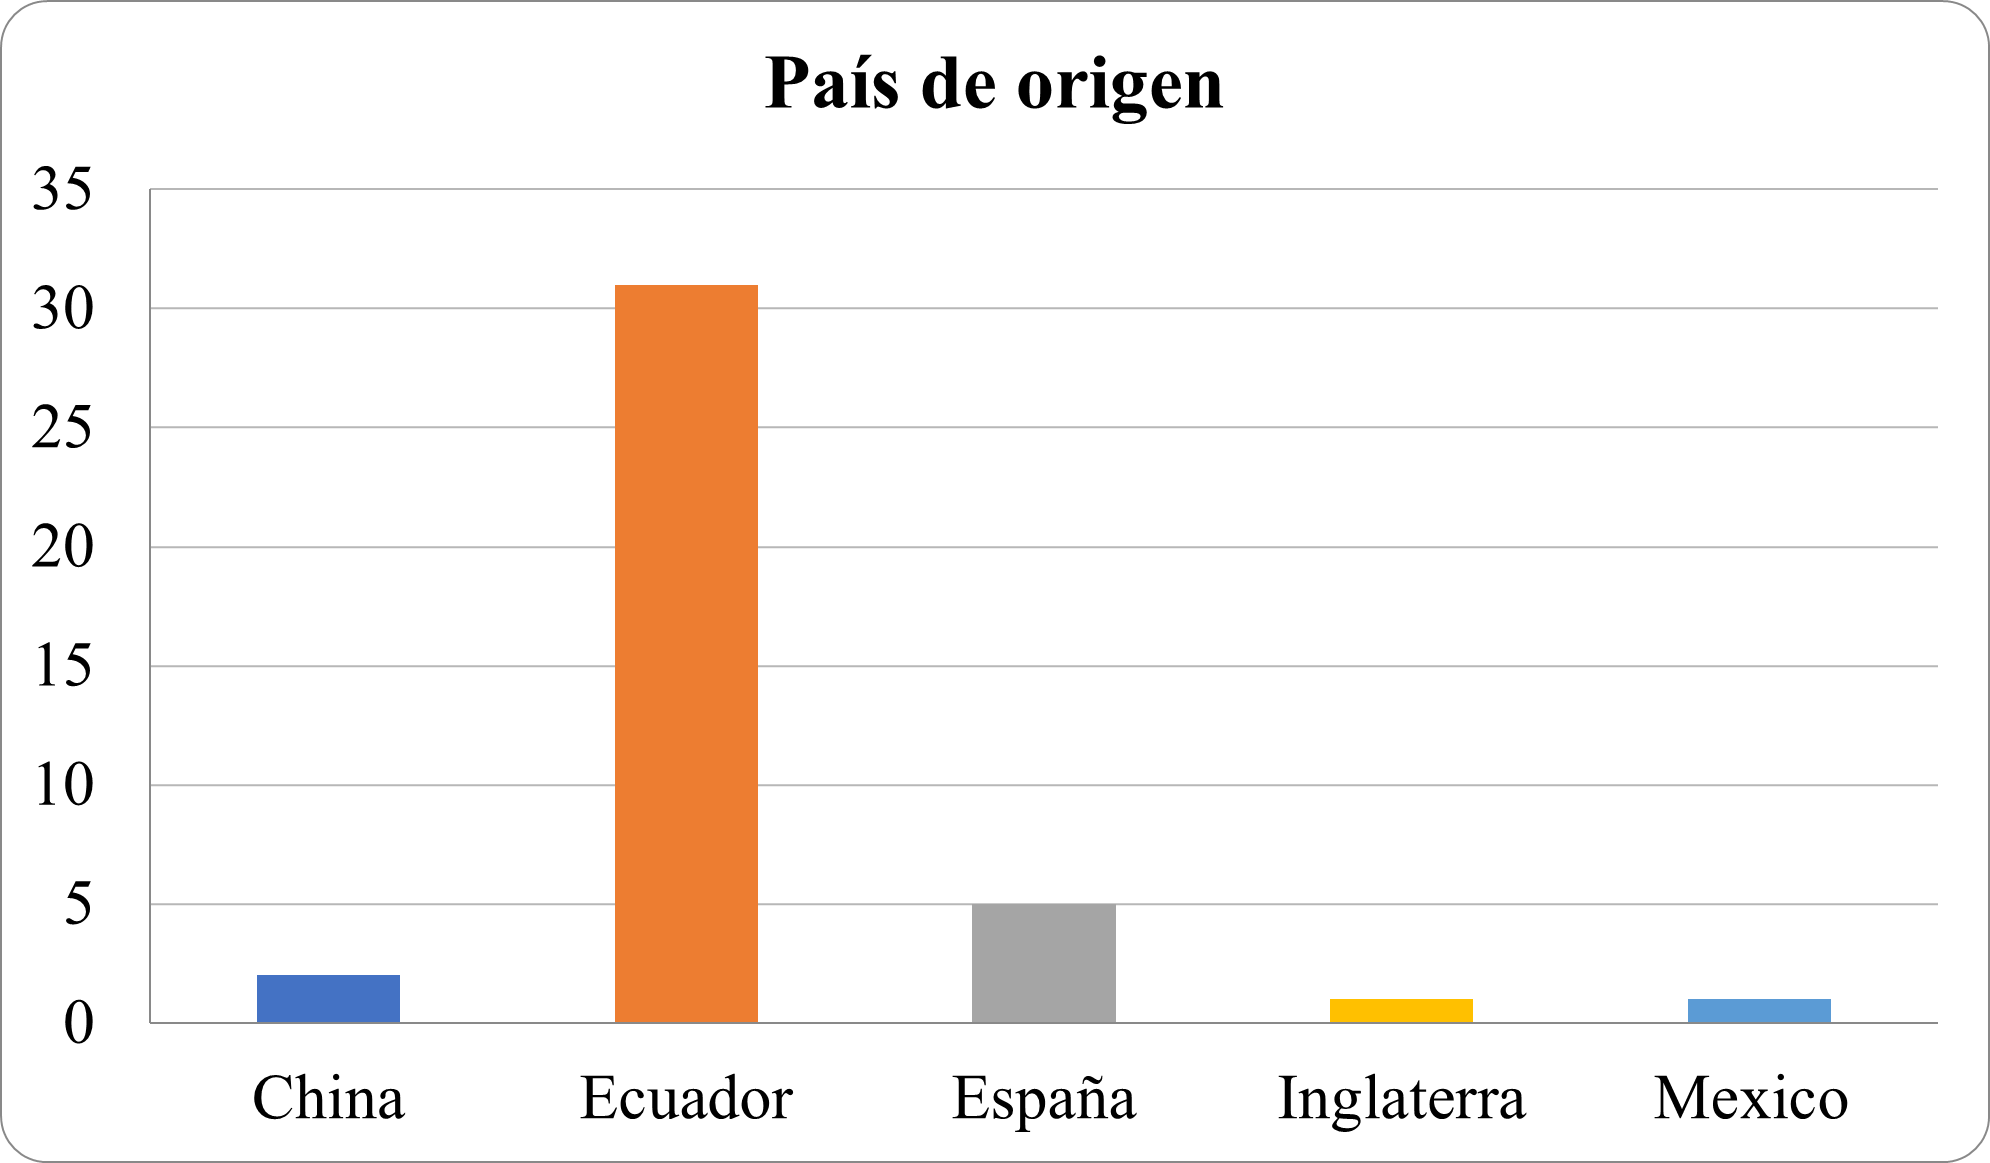
\includegraphics[width=0.9\textwidth]{Graficos/Pais de origen.png }
    \caption{País de origen}
    \label{fig:grafico}
\end{figure}
\par %
 
Entre los procedimientos más comunes se encuentran el análisis documental (Figura 4), que fue utilizado en 8 de los trabajos revisados. Este enfoque implica la recopilación y análisis de documentos históricos, registros y fuentes bibliográficas relacionadas con el patrimonio arquitectónico de Ecuador. Asimismo, se observa un número significativo de trabajos que emplearon entrevistas a expertos (5) y estudios de casos (7) para profundizar en la comprensión de los desafíos y oportunidades asociados con la preservación del patrimonio arquitectónico del país.
 
\par %
  \begin{figure} [h!]
    \centering
    \includegraphics[width=0.9\textwidth]{Graficos/Procedimientos de Investigación.png }
    \caption{Procedimientos de Investigación}
    \label{fig:grafico}
\end{figure}
\par % 
Se identificaron en varios trabajos que aplicaron metodologías innovadoras, como la fotogrametría, el modelado BIM (Modelado de Información de Construcción) y la realidad aumentada, para documentar y visualizar el patrimonio arquitectónico de Ecuador de manera más precisa y detallada. Estas herramientas tecnológicas emergentes están demostrando ser valiosas para la conservación y gestión del patrimonio arquitectónico al proporcionar nuevas formas de documentación, análisis y difusión de la información arquitectónica.

El modelado BIM es una metodología que permite crear modelos digitales tridimensionales de edificios y estructuras, integrando información sobre geometría, componentes, materiales, relaciones espaciales y otros datos relevantes durante todo el ciclo de vida de un proyecto arquitectónico\cite{art:articulo10} Este enfoque colaborativo facilita una mejor comprensión y gestión del patrimonio arquitectónico al proporcionar una representación virtual detallada y precisa de los elementos arquitectónicos, lo que permite realizar análisis, simulaciones y evaluaciones de manera más eficiente y precisa. Además, el modelado BIM facilita la interoperabilidad entre diferentes disciplinas y profesionales involucrados en la conservación y gestión del patrimonio arquitectónico, lo que contribuye a una toma de decisiones más informada y coordinada.
\par %
 \subsection{\textbf{Preguntas de la investigación}}  
\subsubsection{\textbf{¿Cuáles fueron los estilos arquitectónicos predominantes en los patrimonios arquitectónicos de Ecuador y cómo se reflejaron en su diseño y estructura?}}
\par % \cite{art:articulo1}
Los resultados muestran una diversidad de estilos arquitectónicos en el patrimonio de Ecuador, destacando la influencia colonial, republicana, indígena, entre otros. Estos estilos se reflejan en la distribución espacial y uso de materiales. Sin embargo, algunos trabajos señalan desafíos en la conservación debido al deterioro de estructuras históricas \cite{art:articulo18} La diversidad en la tipología arquitectónica revela la influencia de diversos estilos y corrientes arquitectónicas en el país, siendo importante para entender la historia, cultura y guiar las acciones de conservación del patrimonio arquitectónico \cite{art:articulo17}
\par %
En los estilos, nos presenta la tipología arquitectónica, Mismas que se identificaron 85 categorías distintas que abarcan una amplia gama de edificaciones y espacios, desde edificios históricos y religiosos hasta viviendas vernáculas y patrimoniales. Este análisis presenta la complejidad y la riqueza del patrimonio arquitectónico ecuatoriano, que refleja tanto la diversidad cultural del país como su historia y evolución a lo largo del tiempo \cite{art:articulo19}. Entre las categorías más prominentes se encuentran los edificios históricos, religiosos y públicos, así como las viviendas vernáculas y el patrimonio cultural en general (Figura 5)\cite{art:articulo20}.
\par %
La comprensión de estos estilos arquitectónicos es importante para entender la historia y la cultura del país, así como para guiar las acciones de conservación y gestión del patrimonio arquitectónico.
 \par %
  \begin{figure} [h!]
    \centering
    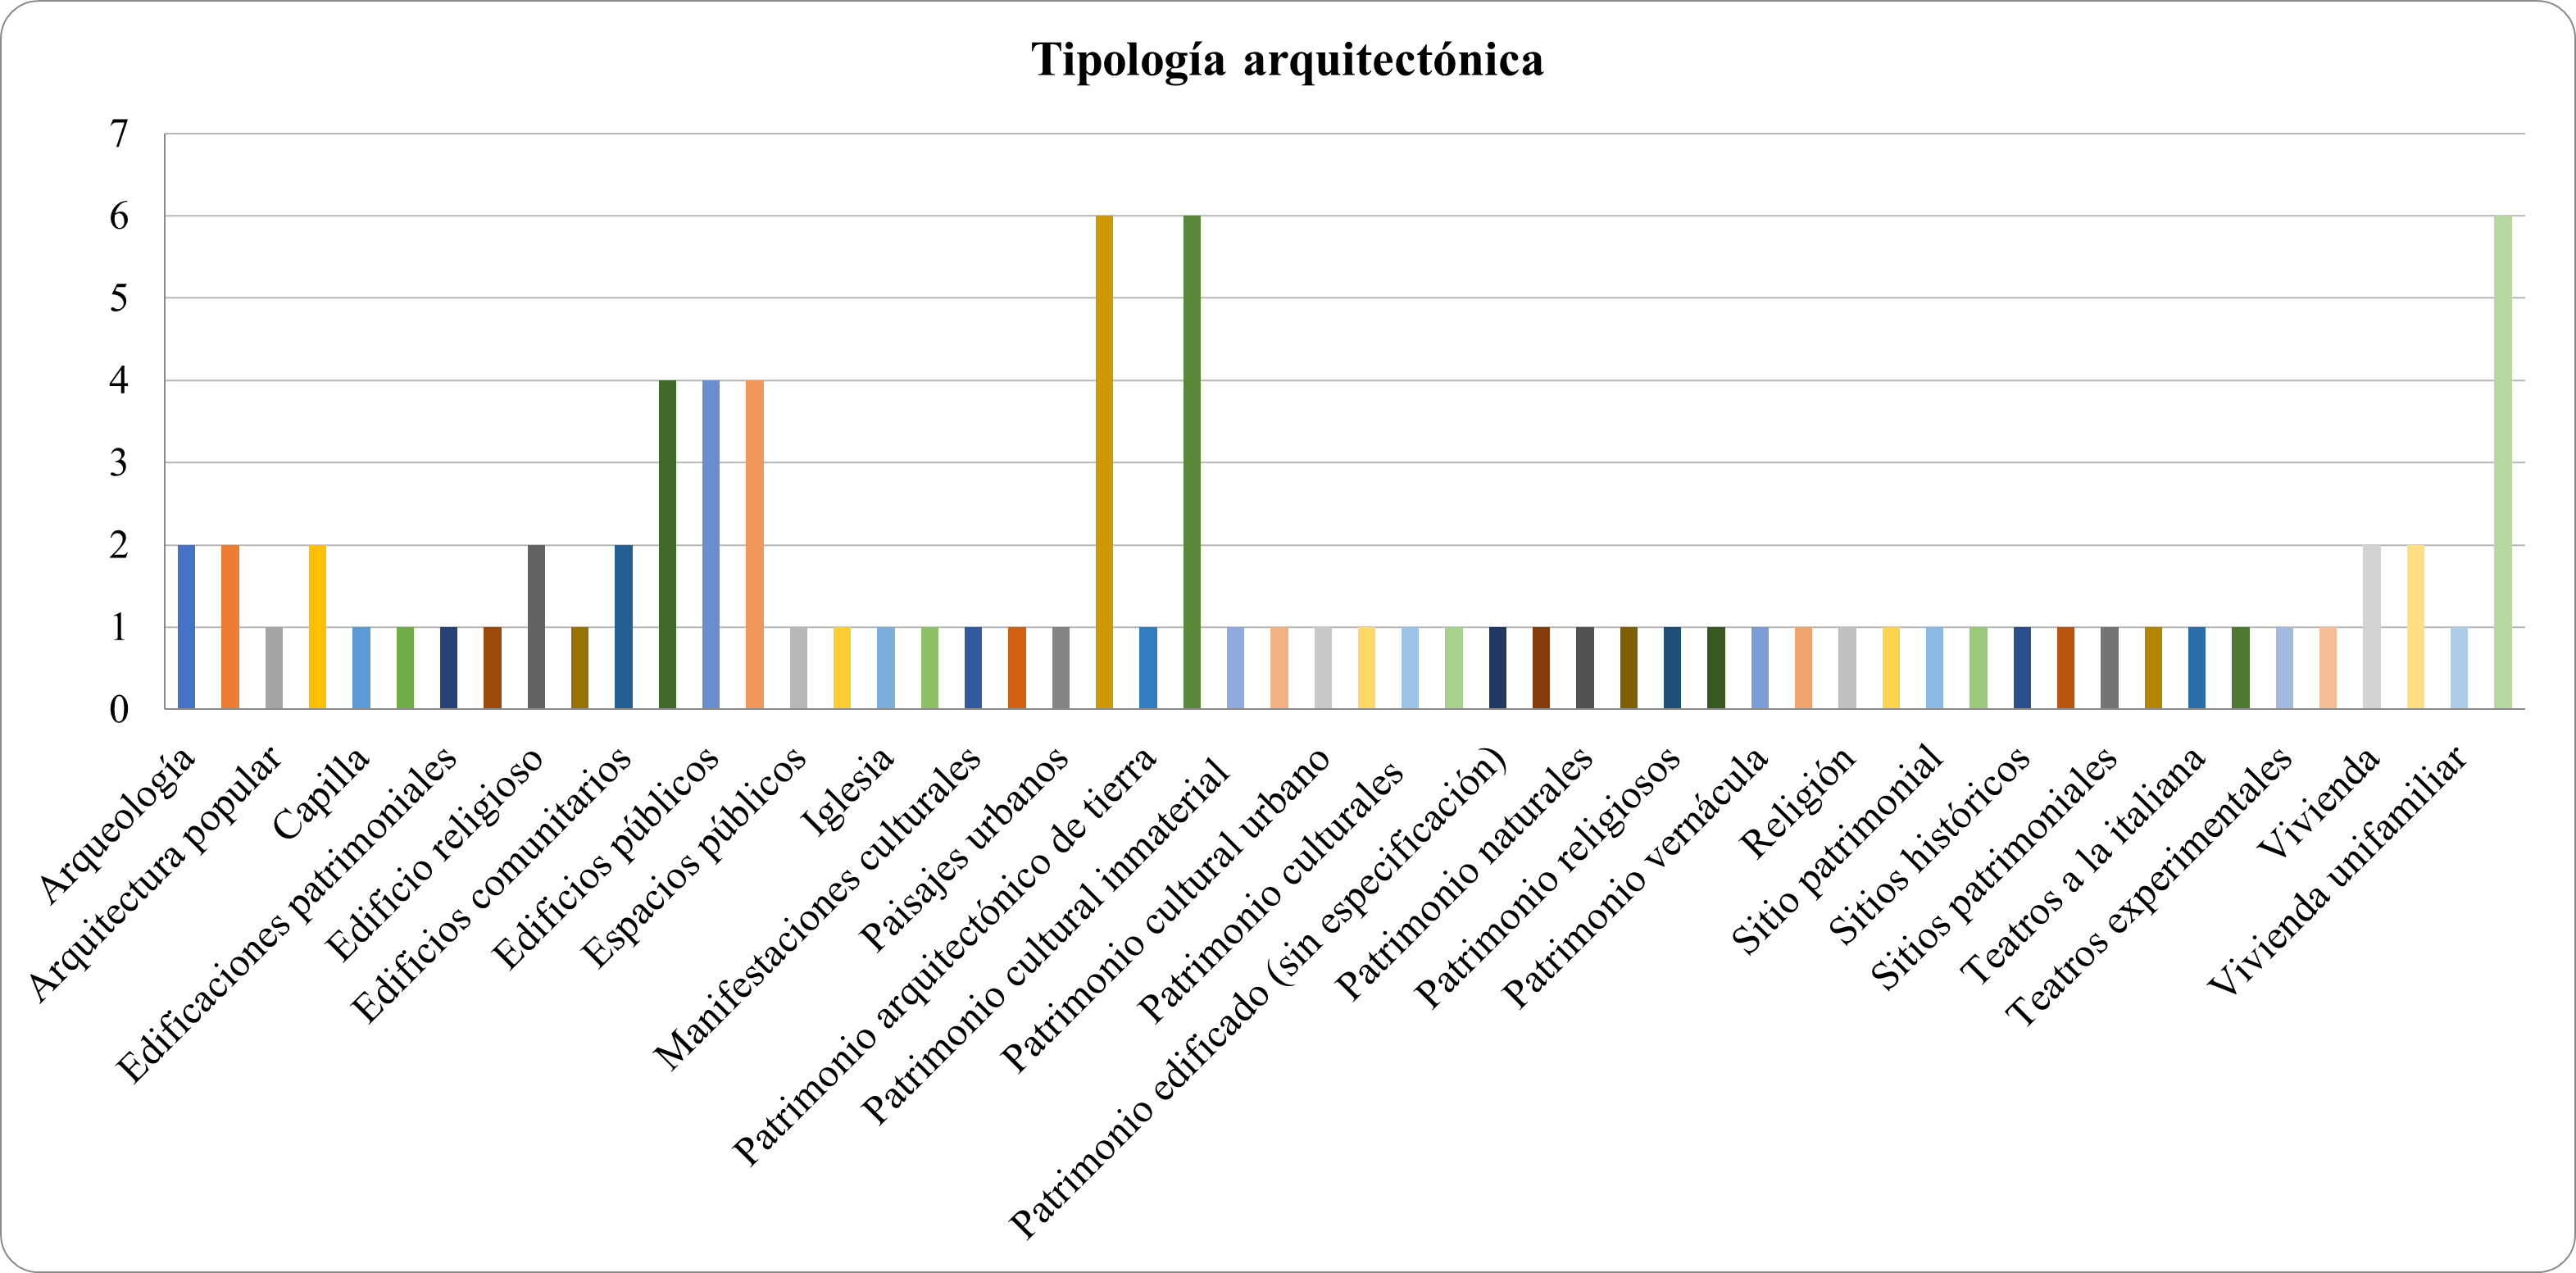
\includegraphics[width=0.9\textwidth]{Graficos/Tipología arquitectónica.png }
    \caption{Tipología arquitectónica}
    \label{fig:grafico}
\end{figure}
\par % 
Por otra parte, se encontraron un total de 84 categorías diferentes, que van desde la arquitectura colonial y republicana hasta el modernismo y el eclecticismo. Entre los estilos más destacados se encuentran la arquitectura colonial, que representa una influencia significativa en el patrimonio arquitectónico de Ecuador, así como el vernáculo, que refleja las tradiciones y prácticas constructivas locales. Estos hallazgos subrayan la importancia de reconocer y preservar la diversidad cultural y arquitectónica del país, así como la necesidad de desarrollar estrategias de conservación que valoren y protejan este patrimonio único (Figura 6).
 \par %
  \begin{figure} [h!]
    \centering
    \includegraphics[width=0.9\textwidth]{Graficos/Estilos y Corrientes Arquitectónicas.png }
    \caption{Estilos y Corrientes Arquitectónicas}
    \label{fig:grafico}
\end{figure}
\par % 
 
Para una mejor comprensión de estos resultados, se presentan gráficos que resumen la distribución de la tipología arquitectónica, los estilos y corrientes arquitectónicas identificados en los estudios revisados. Este gráfico proporciona una visualización clara de la diversidad y la complejidad del patrimonio arquitectónico de Ecuador, destacando la importancia de este campo de estudio para la preservación, valoración de la cultura y la identidad ecuatoriana.\par % 
 
\subsubsection{\textbf{¿Qué elementos culturales y simbólicos estuvieron presentes en los patrimonios arquitectónicos ecuatorianos y cómo contribuyeron a su identidad y significado para la comunidad?}}\par %
Se han identificado una serie de elementos culturales y simbólicos que están incorporados en estas estructuras, y que contribuyen significativamente a su identidad y significado para la comunidad. Este análisis revela la conexión entre el patrimonio arquitectónico y la cultura ecuatoriana, así como la importancia de estos elementos en la preservación y apreciación del legado histórico del país. Dentro del campo de los aspectos culturales incorporados, se destacan diversas categorías que abarcan desde la cosmovisión andina hasta las prácticas sociales y los valores históricos. En total, se identificaron 125 elementos culturales presentes en los patrimonios arquitectónicos ecuatorianos, lo que refleja la diversidad y la riqueza de la cultura del país (Figura 7). 
 \par %
  \begin{figure} [h!]
    \centering
    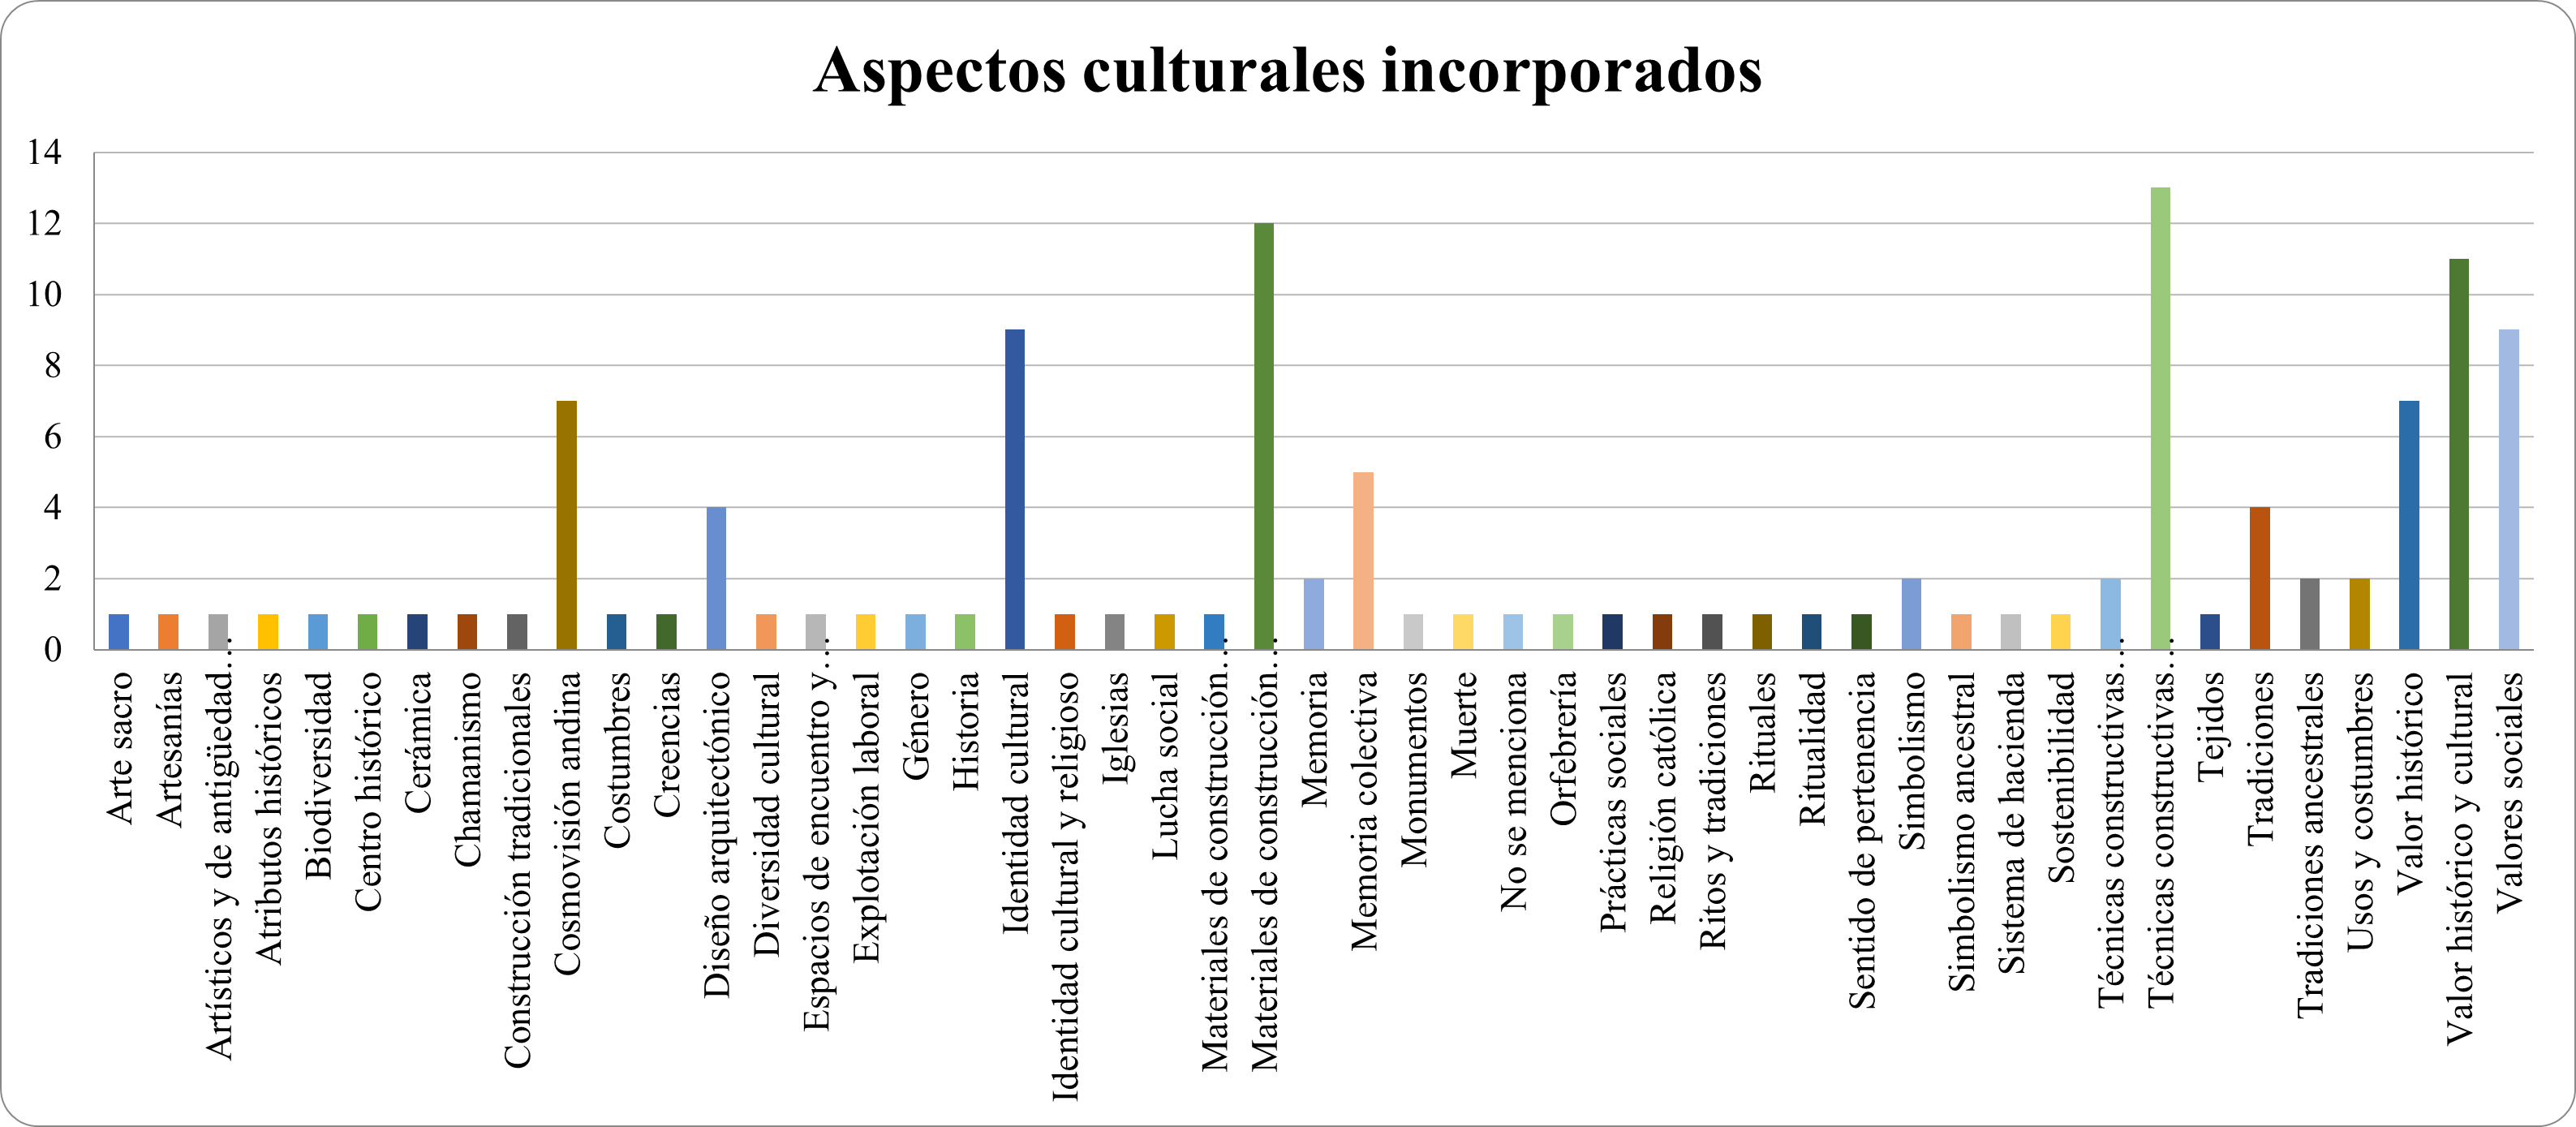
\includegraphics[width=0.9\textwidth]{Graficos/Aspectos culturales incorporados.png }
    \caption{Aspectos culturales incorporados}
    \label{fig:grafico}
\end{figure}
\par % 
Estos elementos no solo proporcionan una conexión con las creencias y prácticas culturales de las comunidades, sino que también contribuyen a fortalecer su sentido de pertenencia y su identidad cultural. Otro aspecto importante es el valor histórico y cultural de estos patrimonios arquitectónicos, que se manifiesta en la preservación de monumentos históricos, la memoria colectiva y la transmisión de tradiciones ancestrales de generación en generación. Estos elementos no solo son testimonios de la historia del país, sino que también son fundamentales para comprender la identidad y la diversidad cultural de Ecuador.
 \par %
\subsubsection{\textbf{¿Cuáles fueron las oportunidades existentes para la conservación y gestión de los patrimonios arquitectónicos ecuatorianos, tales como la implementación de programas de rehabilitación, la promoción del turismo cultural o la participación comunitaria en su preservación?}}\par %
Estos hallazgos ofrecen una visión integral de los materiales utilizados en la construcción, la condición de preservación y los desafíos y problemas que enfrentan estos patrimonios arquitectónicos. En los materiales utilizados en la construcción, se han identificado un total de 183 materiales diferentes, destacando la presencia significativa de materiales tradicionales como la madera, el adobe y la piedra. Estos materiales no solo son parte integral de la arquitectura ecuatoriana, sino que también representan una oportunidad para la preservación de técnicas constructivas tradicionales y la conservación del patrimonio cultural.
 \par %
  \begin{figure} [h!]
    \centering
    \includegraphics[width=0.9\textwidth]{Graficos/Materiales utilizados en la Construcción.png }
    \caption{Materiales utilizados en la Construcción}
    \label{fig:grafico}
\end{figure}
 
En lo que respecta a la condición de preservación, se observa una amplia variedad de estados, desde estructuras en buen estado hasta aquellas en riesgo de colapso o en estado avanzado de deterioro. Esto resalta la necesidad de intervención y estrategias de conservación para garantizar la preservación a largo plazo de estos patrimonios arquitectónicos.
 \par %
  \begin{figure} [h!]
    \centering
    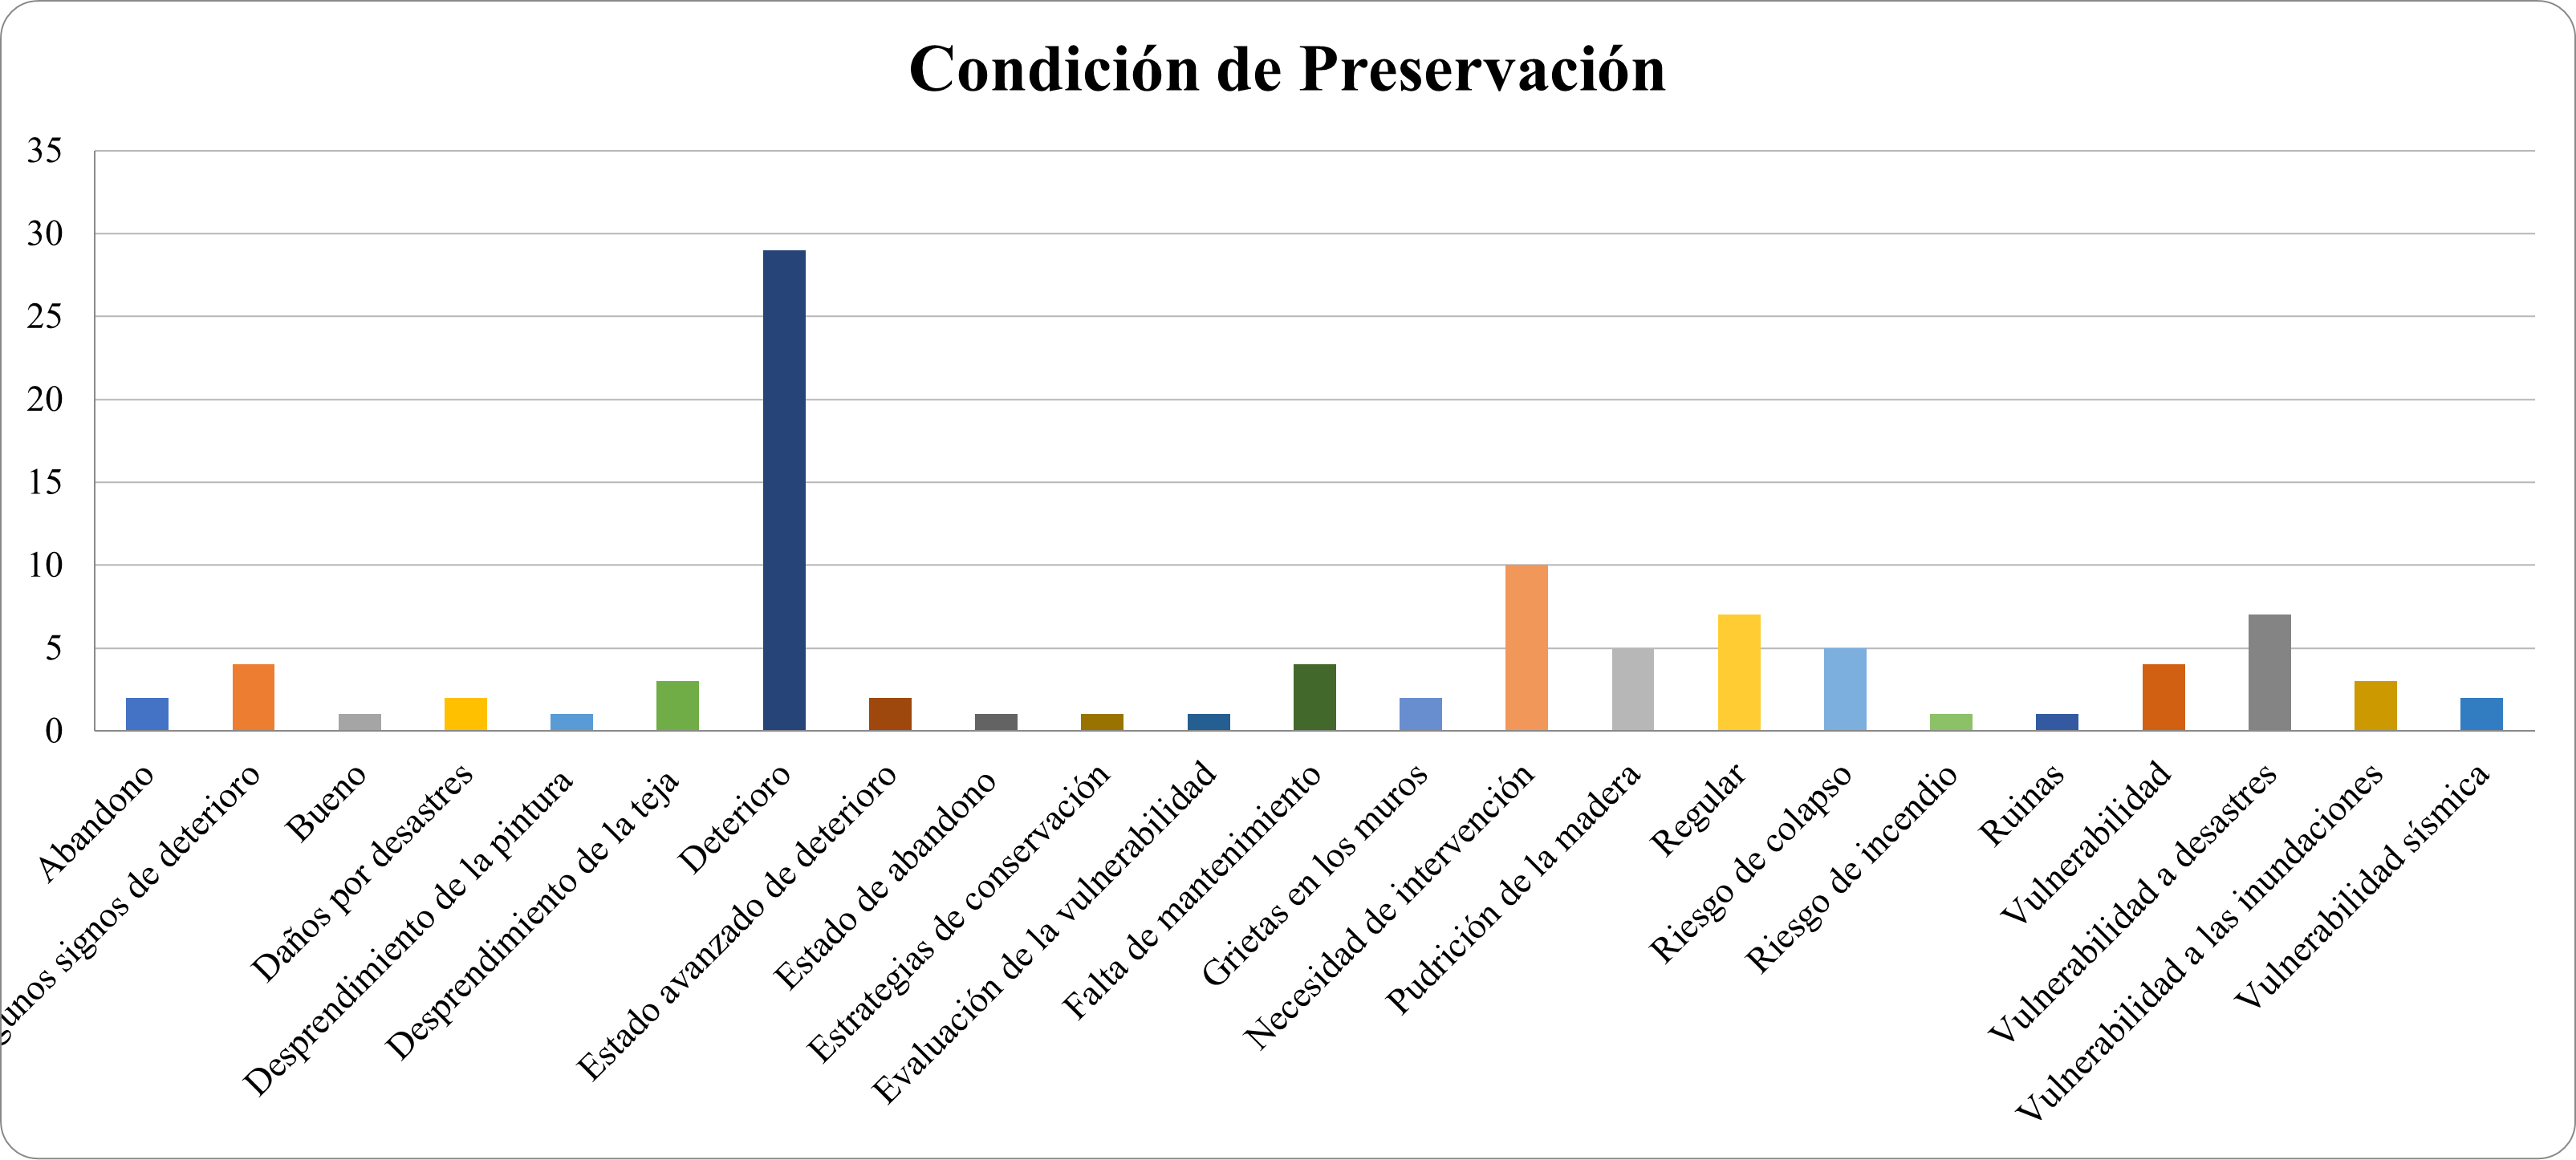
\includegraphics[width=0.9\textwidth]{Graficos/Condición de Preservación.png }
    \caption{Condición de Preservación}
    \label{fig:grafico}
\end{figure}
\par % 
Por otro lado, los desafíos y problemas de preservación identificados son diversos y van desde la falta de recursos y financiación hasta el desinterés político y el vandalismo. Estos desafíos subrayan la importancia de abordar de manera integral la gestión del patrimonio arquitectónico, involucrando a múltiples actores y desarrollando estrategias sostenibles a largo plazo.
 \par %
  \begin{figure} [h!]
    \centering
    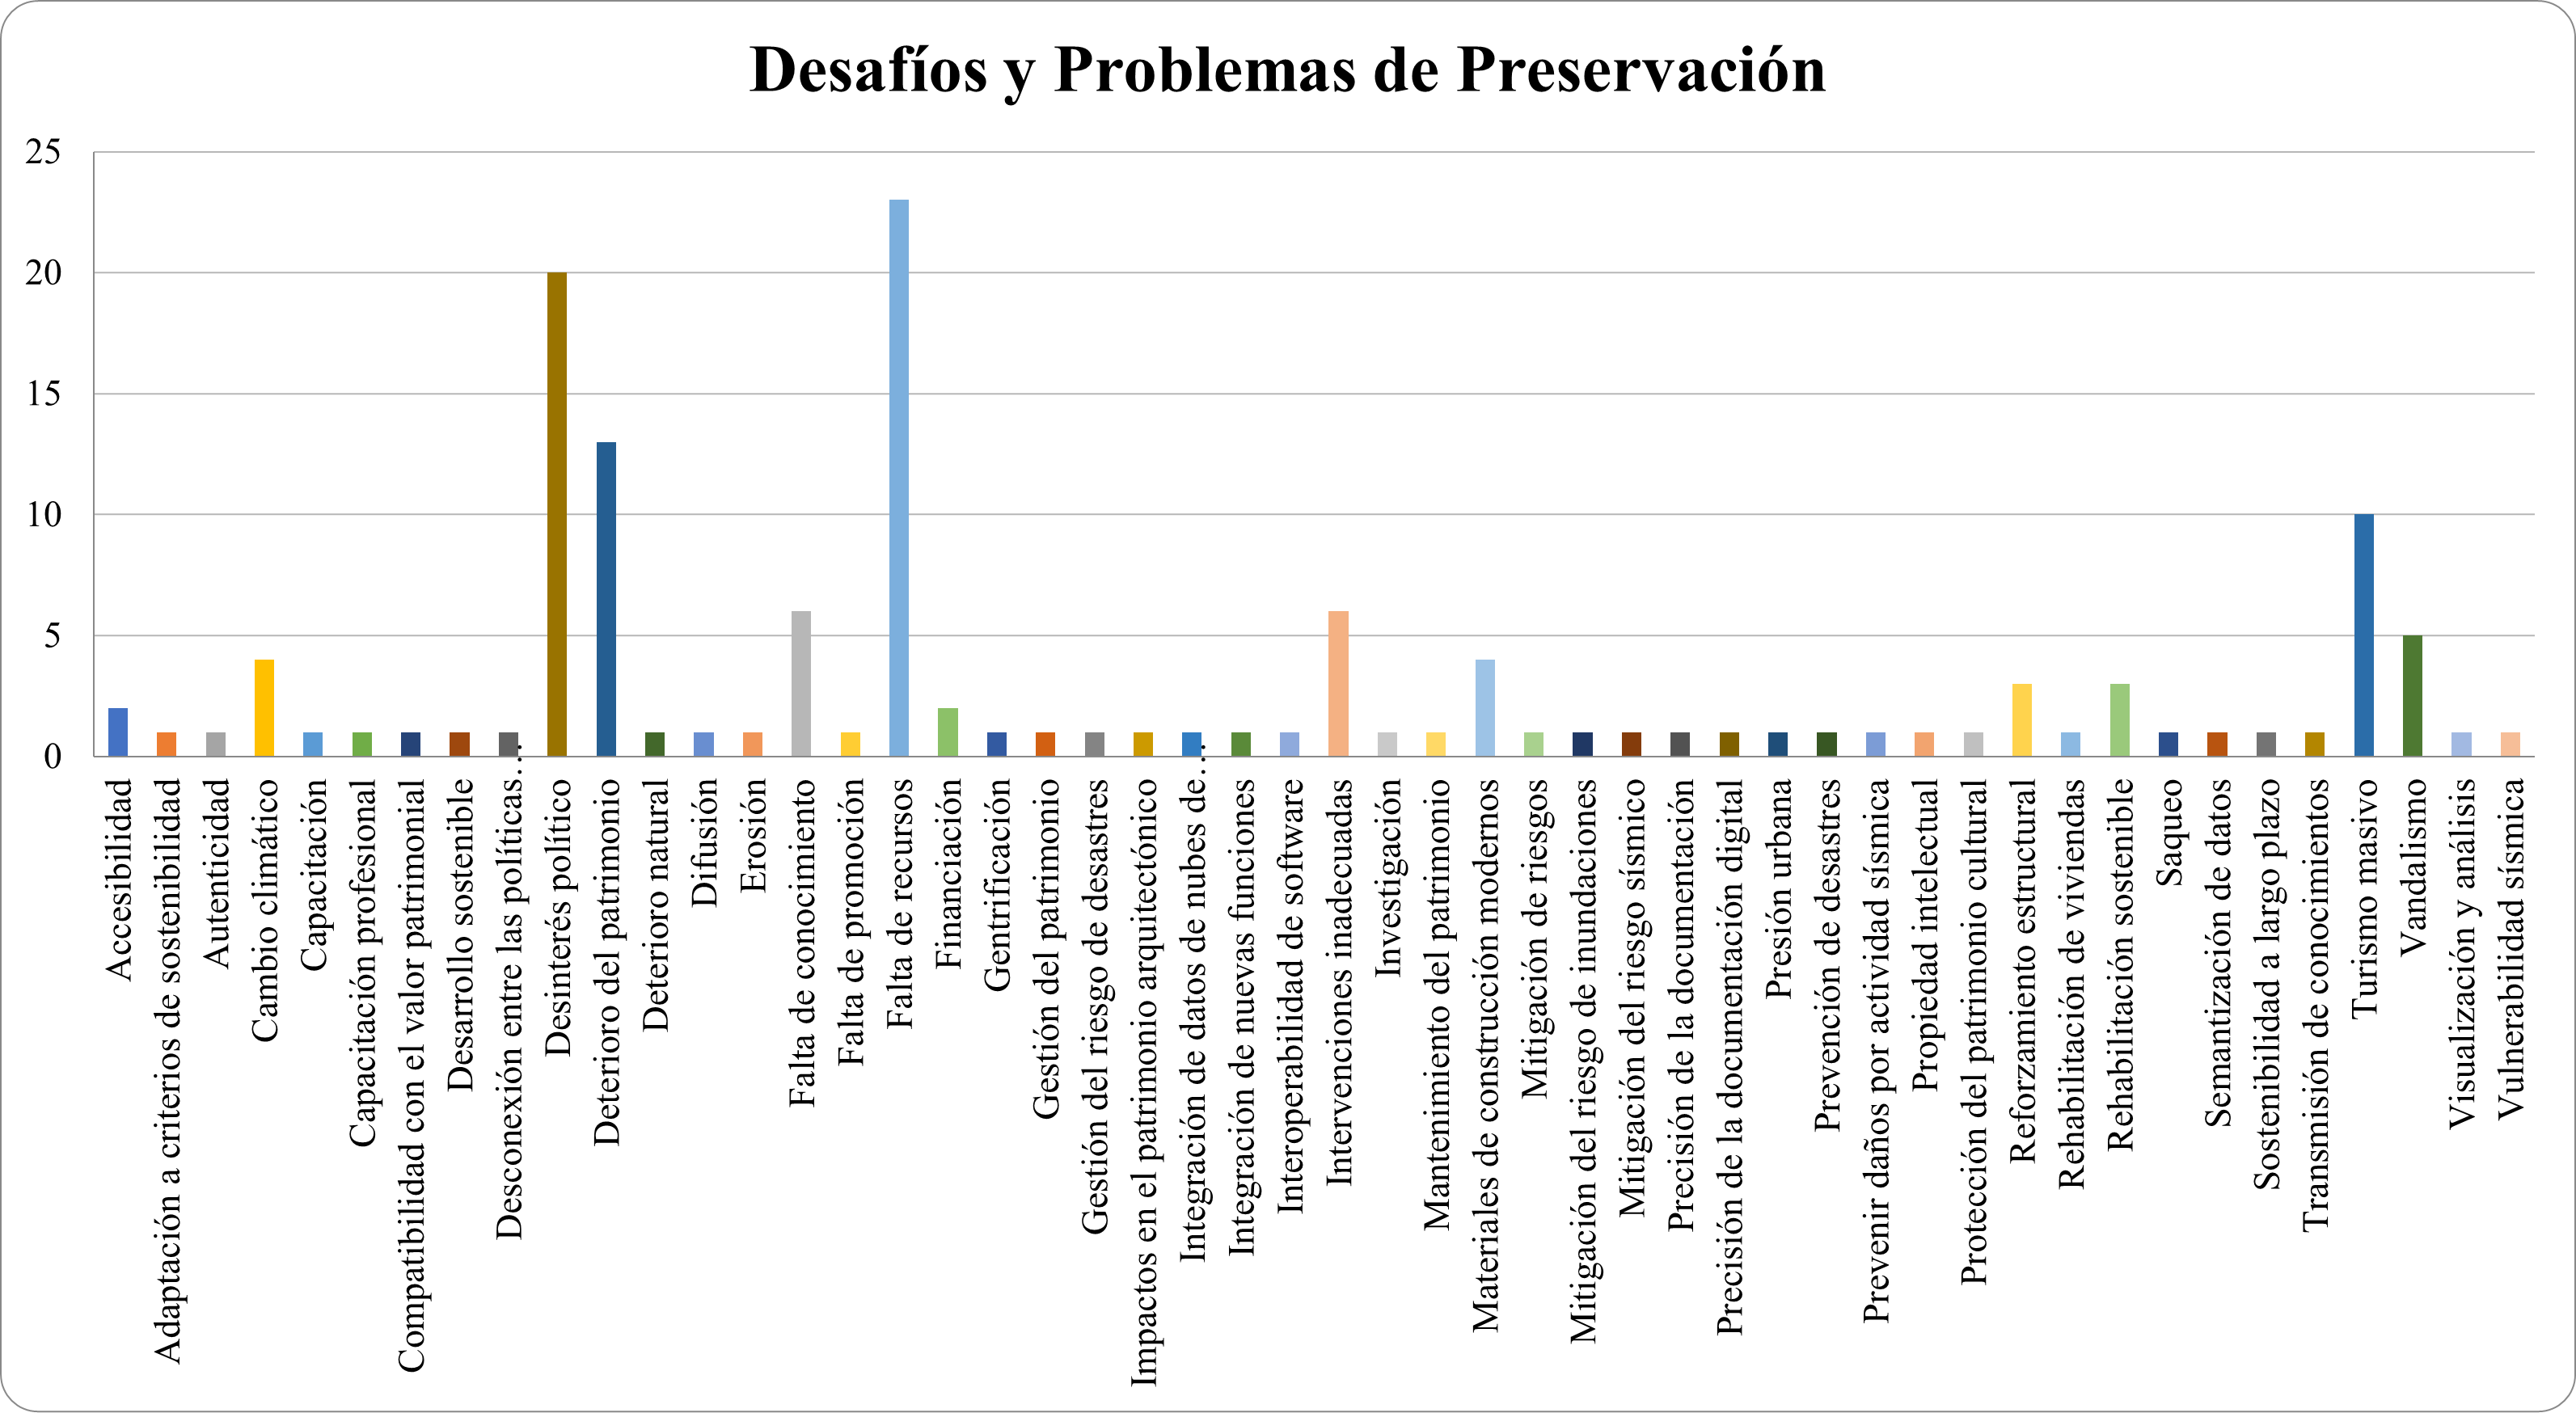
\includegraphics[width=0.9\textwidth]{Graficos/Desafíos y Problemas de Preservación.png }
    \caption{Desafíos y Problemas de Preservación}
    \label{fig:grafico}
\end{figure}
\par %  
 
%%%%%%%%%%%%%%%%%%%%%%%%%%%%%%%%%%%%%%%%%%
\section{ Conclusión}
A través de la síntesis y análisis de estudios previos, se han identificado tendencias  y áreas de interés que requieren una atención continua y un enfoque multidimensional. Se destaca la importancia del patrimonio arquitectónico como elemento fundamental de la identidad cultural y la historia de Ecuador. Las investigaciones revisadas han presentado la necesidad de preservar y valorar estos bienes como parte integral del legado cultural del país, reconociendo su contribución a la identidad nacional y al bienestar de las comunidades locales.

Por otro lado, se ha evidenciado que el patrimonio arquitectónico enfrenta desafíos, incluida la degradación física, la pérdida de autenticidad, la presión urbana y los riesgos ambientales. Estos desafíos requieren estrategias de conservación y gestión que sean holísticas, adaptativas y sostenibles, incorporando enfoques interdisciplinarios y la participación activa de la comunidad.

Además, se ha resaltado el papel de la participación comunitaria y la educación pública en la conservación del patrimonio arquitectónico. La investigación ha demostrado que la participación efectiva de las comunidades locales y la sensibilización pública son fundamentales para el éxito de los proyectos de conservación, promoviendo una mayor conciencia y aprecio por el valor del patrimonio histórico.

Asimismo, se ha reconocido el potencial del turismo cultural como una fuente de financiamiento para la conservación del patrimonio arquitectónico, que requiere un enfoque equilibrado de la sostenibilidad y la preservación de los sitios patrimoniales, minimizando los impactos negativos asociados al turismo masivo.

%%%%%%%%%%%%%%%%%%%%%%%%%%%%%%%%%%%%%%%%%%
\section{ Agradecimientos }
En nombre de los cuatro autores de esta revisión sistemática sobre los Patrimonios Arquitectónicos de Ecuador, se expresa el más sincero agradecimiento a los investigadores, académicos y expertos cuyos estudios y publicaciones formaron la base del análisis. Sus contribuciones fueron fundamentales para el desarrollo de esta investigación y para alcanzar una comprensión más profunda del tema.

Además, se reconoce el apoyo brindado por el docente de la materia de Fundamentos de redacción científica, quien ofreció orientación, comentarios y sugerencias durante todo el proceso de investigación. Su colaboración fue invaluable para la comprensión del tema y mejorar la calidad del trabajo realizado.

%%%%%%%%%%%%%%%%%%%%%%%%%%%%%%%%%%%%%%%%%%
\begin{adjustwidth}{-\extralength}{0cm}
%\printendnotes[custom] % Un-comment to print a list of endnotes
 
\reftitle{Referencias}

 \nocite{*} 
\bibliographystyle{IEEEtran}
\bibliography{references.bib}
 
\end{adjustwidth}
\end{document}

